% !TEX TS–program = pdflatexmk
%%%%%%%%%%%%%%%%%%%%%%%%%%%%%%%%%%%%%%%%%%%%%%%%%%%%%%%%%%%
% EPFL report package, main thesis file Goal: provide formatting for theses and
% project reports Template's Author: Mathias Payer <mathias.payer@epfl.ch>
% Thesis's Author : Arnaud Pannatier <arnaud.pannatier@epfl.ch>
%%%%%%%%%%%%%%%%%%%%%%%%%%%%%%%%%%%%%%%%%%%%%%%%%%%%%%%%%%%
\documentclass[a4paper,11pt,oneside]{report}
% Options: MScThesis, BScThesis, MScProject, BScProject
\usepackage[MScThesis]{EPFLreport} \usepackage{xspace}
\usepackage{array}
\usepackage{rotating}
\usepackage{placeins}
\newcommand{\PreserveBackslash}[1]{\let\temp=\\#1\let\\=\temp}
\newcolumntype{C}[1]{>{\PreserveBackslash\centering}p{#1}}
\newcolumntype{R}[1]{>{\PreserveBackslash\raggedleft}p{#1}}
\newcolumntype{L}[1]{>{\PreserveBackslash\raggedright}p{#1}}
\usepackage{arydshln}


\usepackage{booktabs}
\usepackage{caption}
\usepackage{float}
\usepackage{titlesec}
\usepackage{capt-of}

%dashed line
\usepackage{array}
\usepackage{arydshln}
\setlength\dashlinedash{0.2pt}
\setlength\dashlinegap{1.5pt}
\setlength\arrayrulewidth{0.3pt}

%Widows & Orphans & Penalties
\widowpenalty500
\clubpenalty500
\clubpenalty=9996
\exhyphenpenalty=50 %for line-breaking at an explicit hyphen
\brokenpenalty=4991
\predisplaypenalty=10000
\postdisplaypenalty=1549
\displaywidowpenalty=1602
\floatingpenalty = 20000

\title{A Control Plane in Time and Space for Locality-Preserving Blockchains}
\author{Arnaud Pannatier}
\supervisor{Cristina Basescu}
\adviser{Prof. Bryan Ford}
%\coadviser{Second Adviser}
\expert{\color{red}The External Reviewer\color{black}}

\newcommand{\sysname}{FooSystem\xspace}

\begin{document}

\maketitle 

\maketoc

%%%%%%%%%%%%%%%%%%%%%%%%%%%%%%%%%%%%%%%%%%%%%%
\chapter{Introduction} %%%%%%%%%%%%%%%%%%%%%%%%%%%%%%%%%%%
%%%%%%%%%%%%%%%%%%%%%%%%%%%%%%%%%%%%%%%%%%%%%%

%% Presentation and setting
Distributed ledgers were the trend of the last ten years. You might realize
that when your hairdresser starts to tell you that he plans to put his money
into blockchains or when your little cousin asks to have some Bitcoin
\cite{Nakamoto2009} for Christmas. The research in this field is growing every
year. However, distributed ledgers still have weaknesses. The purpose of this
work is to propose a solution concerning two well-known weaknesses. The first
one is the time required to confirm a transaction.  Indeed, in Bitcoin
\cite{Nakamoto2009}, validating a transaction can take around one hour, because
it takes around ten minutes to validate a block, and it needs around six blocks
to be convinced with a high probability that the ledger won't be forked, and
the transaction invalidated. This might be okay for some transactions of great
value. For example, if somebody is buying a car using Bitcoin
\cite{Nakamoto2009}, this person might agree to wait one hour so that its
transaction is validated. However, if somebody wants to use it to buy its daily
coffee, it might be a bit annoyed with this waiting time. The other weakness
appears in World War III scenarios. If a third World War occurs, splitting the
world in two, one can expect that the communication between the two sides might
be cut. This is a problem for regular distributed ledger as it will lead to
forks that cannot be resolved at the end of World War III. This work is part of
a bigger project called Nyle [\autoref{fig:Nyle}], which uses the idea of
locality to solve these problems.  The idea is to replicate the system along
regions of different sizes, from local (e.g. Switzerland, London) to global.
With this idea, a transaction can be validated in a local region first, but it
is still possible to wait for global validation if needed. Most of the time a
transaction that was validated locally will be validated globally as well, but
in some case, when propagating the information to the global regions, some
transactions might be invalidated as they are in conflicts with others,
therefore one or both won't be accepted to avoid double-spending. For big
transactions, people might prefer to wait for global confirmation. But if one
wants to buy its daily coffee, local validation might be enough for the
merchant, especially if he knew already the person. For World War III
Scenarios, Nyle offers a solution as well, indeed if a global partition occurs,
the system replicated in smaller regions that are not split
by a partition can continue working flawlessly. 

\begin{figure}[!h]
\centering
\includegraphics[width=400pt]{figures/Nyle}
\caption{Sketch of Nyle: The Blockchain is replicated across all region}s
\label{fig:Nyle}
\end{figure}

%% Main Challenge
Nyle's distributed ledger is maintained by nodes that are spread over the
world.  Clients will then ask the nodes to proceed with their transactions or
other requests. Nodes are participating in a different number of regions. A
first challenge is to draw these regions adequately. A second problem is
\textit{open-membership}: it should be possible for anybody with sufficient
computational power and a good connection to maintain a node of the system.
This allows the system to be distributed. The challenge with
\textit{open-membership} is that there should be a way to know the participants
of the system if one wants to have a consensus.  A second challenge is that
nodes can join, leaves or move in the system at any moment. This might not be a
problem for classic distributed ledger as Bitcoin \cite{Nakamoto2009}, as its
protocol only takes into account the computational power that is in the system
at a given time. But as Nyle is locality-based, this might lead to additional
challenges, each corresponding to the different actions possible: joining,
leaving and moving. For joining nodes, consider the case where there were only
a few nodes spread along a big region, for example, Western Europe, and after a
while, a large number of new nodes wants to join there. If the region stays the
same, this might lead to some problems, indeed the consensus would take more
time and the liveness could not be guaranteed. Furthermore, for a region of
this size, the probability of a partition is relatively important.  One might
want that in this case, additional regions with the side of countries would be
created. This leads to the idea that the regions should be able to adapt
depending to node membership. If nodes leave the system, this might lead to
problems as well. Indeed in the opposite situation as before, after a while,
some regions might not contain any nodes that are maintaining the system. To
avoid this situation, one might want to modify the regions when nodes leave to
guarantee that a sufficient number of nodes are in a region at any time. Moving
nodes are creating problems as well if the region assignment is fixed but the
nodes are moving, a node drifts apart after a while far away from the region it
was assigned to. This might take a while, but one can imagine the situation
where a lot of nodes have moved far away from their original position. In case
of a global partition, this can lead to the failure of even small regions, that
is one problem that one wants to avoid in Nyle. Therefore the regions should be
adapted with the movement of the nodes. 

%% Related Work Is Insufficient
Most of this work is based on the CRUX \cite{Basescu2014}, which introduces the
an algorithm that allows creating regions based on compact graph theory and
which is described in more detail in \autoref{chap:Background} and which
provides the existing code base in Go. The existing work on Nyle was done by
Maxime Sierro and Cristina Basescu \cite{Sierro2019} which proposes the first
implementation of Nyle building on the top CRUX \cite{Basescu2014} but focusing
directly on how to improve the storage of the transactions and the tree
structure of the regions. This work builds directly upon the existing work, but
is slightly orthogonal, as the Control Plane is not directly linked to the
replicated blockchain. A second work on Nyle, called \textit{proof-of-location}
was done by Sabrina Kall \cite{Kall2019}, which was proposing a way of checking
efficiently the location of a node and to assert if nodes were lying about the
the location where they claimed to be. There is a current work by Guillaume
Michel on the Interplanetary-File System (IPFS) \cite{Michel2019}, that is
based on CRUX as well but with the purpose to create a locality-aware overlay
to speed the system up, but it is not directly related to blockchains. The rest
of the related work is described in the next chapter \autoref{chap:RelatedWork}
and is mostly orthogonal to the current approach: some other solutions to speed
the validation of transaction are Bitcoin \cite{Nakamoto2009}, Byzcoin
\cite{Kogias2016}, Omniledger \cite{Kokoris-Kogias2017}, DFINITY
\cite{Hanke2018}, Monoxide \cite{Wang2019} and Stellar \cite{Lokhava2019}, but
they don't use the concept of the locality for this purpose. 

%% Description of the Approach
This work was structured in the following manner: first, a simple version of
the control plane was designed \autoref{chap:Design}, which splits the time
into epochs and take as an assumption that the system is fixed during one
epoch. A protocol is proposed and discussed and the threat analysis is done.
Based on its implementation and performance analysis some drawbacks are put
into light.  Then a series of strawman models try to correct some of these
drawbacks and are analyzed as well \autoref{chap:Improvements}. The first one
is called "Locarno Treaties" and will try to keep the system coherent from one
epoch to the next.  The next one is called "Fog of the war", and try to reduce
the need for communication between nodes. The last and the most complex
Strawman considers the interactions of the nodes as a space-time graph and try
to build upon the existing patterns that appear in these graphs to propose a
different notion of distance. 

%% Why it is needed.
%% Already discussed in Main challenges so it is merged with the next

%% Thesis Statement
This work proposes \textbf{A Control Plane in Time and Space for
Locality-Preserving Blockchains}. This control plane for Nyle is needed to
ensure to have a \textit{open-membership} and to solve the problems of World
War III scenarios and to allow regional validations. The series of strawman
models improving the simple control plane leads to the use of Space-Time graphs
that allowed to improve the existing design. 

%% Results 

%%My Contribution

%%%%%%%%%%%%%%%%%%%%%%%%%%%%%%%%%%%%%%%%%%%%%%
\chapter{Related Work} \label{chap:RelatedWork} %%%%%%%%%%%%%%%%%%%%%
%%%%%%%%%%%%%%%%%%%%%%%%%%%%%%%%%%%%%%%%%%%%%%

This work builds upon several other works that are linked to the domains of
blockchains and locality. Nyle proposes a decentralized cryptocurrency using
different strategies than Bitcoin \cite{Nakamoto2009}, Byzcoin
\cite{Kogias2016}, Omniledger \cite{Kokoris-Kogias2017}, DFINITY
\cite{Hanke2018}, Monoxide \cite{Wang2019} and Stellar \cite{Lokhava2019}. But
it used them as a source of inspiration and share some aspects with theses
general cryptocurrencies. It is somehow orthogonal to them because it can use
any of these cryptocurrencies as an underlying system and enhance them using
the idea of the locality to provide them with some partition-resistance and
regional validation. 

Some concepts are directly inspired by these works. The Sybil-resistant scheme
used in the registration system is directly inspired by DFINITY
\cite{Hanke2018}, using \textit{endorsement} in the general way, which can be
in practice replaced by any Sybil-resistance scheme like Proof-of-Work
\cite{Nakamoto2009}, Proof-of-Stake \cite{wood2014ethereum}, or even
Proof-of-Personhood \cite{Borge2017}. In particular, this work tries to solve
some drawbacks of traditional cryptocurrencies like Bitcoin
\cite{Nakamoto2009}, solving the problem of the waiting time for transaction
validation by using regional validation and making it resistant to WWIII
scenarios. Byzcoin \cite{Kogias2016} and Omniledger \cite{Kokoris-Kogias2017}
give another interesting solution to accelerate the validation, but their
results are orthogonal to this research. Stellar's solution for
\textit{open-membership} \cite{Lokhava2019} is based on a quorum, allowing each
node to trust a subset of other nodes of its choice. It is an elegant solution
and permits to validate transactions fast and securely. A certain complexity
seems to be added both in the theoretical and practice part, this justifies why
a similar approach was not followed. However, the idea to allow nodes to have a
different view of the system is at the core of one of the improvements of this
work, described in \autoref{sec:Fog-of-the-war}.

Omniledger \cite{Kokoris-Kogias2017} and Monoxide \cite{Wang2019} use sharding
to increase performance. Sharding splits the system in a random committee that
allows the fastest processing of the transaction. This not directly related to
what is done in this work, as even if the system is split into different parts,
it is not done randomly but based on the locality, and the system is replicated
in all the regions. However, cryptocurrencies using shards can still be used as
an underlying system of Nyle, enhancing the performance of the
partition-resistant blockchain system created by this means.

This work is directly related to the locality-preserving algorithms developed
in CRUX \cite{Basescu2014} and compact-graph algorithms \cite{Thorup2005}.
These are described in detail in \autoref{chap:Background}. There is a class of
algorithm that uses the idea of locality differently. For example, Geo-DNS
\cite{Katz-bassett2006} or IP Anycast \cite{Abley2006} use the locality to
shorten the path for the packets, connecting the servers via the closest path.
Replication is often used to guarantee the integrity of the stored information
\cite{Mokadem2015}. In CRUX \cite{Basescu2014} and Nyle regional replication of
the system is used to create partition-resistance, and in Nyle, it can be used
to allow region validation.

Some classic consensus protocols as PAXOS \cite{Lamport2000}, PBFT
\cite{Castro1999} were used as an inspiration to the protocol. In practice, and
for efficiency, this work uses BlsCoSi \cite{Boneh2018} that is much more
efficient, because it makes smart use of trees for communication.  BlsCoSi
\cite{Boneh2018} is still prone to some failures in case of successive
view-changes, it could be improved using a different protocol such as HotStuff
\cite{Yin2018} which solves the problem of view change using a third round of
communication. 

This work uses a distributed public algorithm for the source of randomness like
Randhound \cite{Syta2016}. Each node will use this source to draw a random
level. The way it is used is described in detail in the next section. 


%%%%%%%%%%%%%%%%%%%%%%%%%%%%%%%%%%%%%%%%%%%%%%
\chapter{Background} \label{chap:Background} %%%%%%%%%%%%%%%%%%%%%%
%%%%%%%%%%%%%%%%%%%%%%%%%%%%%%%%%%%%%%%%%%%%%%

%%%% Plan
% - Crux (??)
% - Nyle (7-8p) - General description - What is already implemented - Next
%  steps
% (motivation for the control plane)
%%%%%%%%%%%%%%%%%%

This Master Thesis is part of a larger project that concerns
locality-preserving systems. In particular, it builds upon
CRUX \cite{Basescu2014} and is part of Nyle. This section describes two
different projects. 

\section{CRUX - Fast and Resilient Datastore with Automated Locality}

%%%% General Presentation
% - Solution to partition
% - General idea
% - Small Overhead
% - Generality 
% - CAP Theorem
%%%%%%%%%%%%%%%%%%
\subsection{Description}
CRUX \cite{Basescu2014} introduces a smart way of dealing with partitions in
decentralized systems. Partitions occur in decentralized systems, but one can
maybe try to find a solution to reduce their effects on the global system. For
example, if a partition occurs, there is no reasons that nodes that are
functioning in the same side of the partition should stop working because of
the partition. 

The general idea is that a system can be replicated at different scales, from
local (big cities, small countries) to global. With the additional property
than each replicated system will continue to work correctly if no partition
splits it. If a global partition occurs, then the global region might not work,
but all the replicated system in local regions will continue working. This is a
direct solution to the previously mentioned problem: nodes working on the same
of the partition will continue to work.

This solution comes with an overhead, as the system should be replicated in all
the regions. But there are some ways of reducing this overhead, in a way that
it stays reasonable and that the resistance to partition is maintained. CRUX
algorithm for regions creation \cite{Basescu2014} presented below ensure that
the proper number of regions is created in a manner that the number of regions
created induces a reasonable overhead and that the partition resistance stays
efficient. If CRUX \cite{Basescu2014} is used for a specific system, overhead
can be even more reduced: as the systems are replicated in every region, most
of the data is replicated as well. So one might dig inside the specification of
one system and manages not to store twice the same data. But this goes beyond
the goal of CRUX \cite{Basescu2014}, which wants to be the more general
possible. 

Indeed, the force of CRUX \cite{Basescu2014} is that it applies to any
distributed system, as no particular hypothesis on the system is made. It only
starts from one simple idea: one system can be replicated at a smaller scale to
ensure some partition resistance. 

% TODO: do more research on that.
A note should be made about the CAP-theorem. Recall that this theorem states
that no system can be consistent, available and partition-resistant at the same
time. It seems that this solution is adding partition tolerance to an available
and consistent system. Thus leading to the violation of the theorem. But it is
not exactly the case, as the enhanced system only ensure that nodes can still
work in some regions that are not affected by the partition. The regions split
by a partition are not working anymore. Even if the system can still work on
the same side of a partition, it's not totally partition resistant.

%%%% Common Tools
% - Approximation distance oracle
% - Bunch
% - Cluster
% - ARA 
%%%%%%%%%%%%%%%%%%
\subsection{Common Tools} \label{sec:common-tools}
This section describes how to create
regions that are used to replicate the system. These regions are used by Nyle
as well, therefore we will describe it in detail. These regions are called
\textit{Available Responsive Areas} (ARA), in each region a copy of the replicated
system is deployed. To create these regions each node will participate first at
a lottery. Each node starts at level 0. Then each node goes to the next level
with a given probability $P$. This
procedure is repeated at each level and is stopped when no nodes are promoted
to the next level. This first empty level is called $K$. Then each node can
compute two quantities that will be necessary to create \textit{ARAs}: their
bunch and their cluster. 
 
 \begin{table*}[h!] \centering
\begin{tabular}{@{}ccccc@{}}\toprule
\textbf{Sample size} & \textbf{Level $\#1$} & \textbf{Level $\#2$} & \textbf{Level $\#3$} & \textbf{Level $\#4$} \\ \midrule
100 & 90 & 9 & 1 & 0 \\ \hdashline
200 & 180 & 18 & 2 & 0\\ \hdashline
 500 & 450 & 45 & 5 & 0\\ \hdashline
 1000 & 900 & 90 & 9 & 1\\ %\hdashline
\midrule
$N, k=2$ & $N(1-p)$ & $Np(1-p)$ & $Np^2$ & $0$ \\ \hdashline
$N, k=3$ & $N(1-p)$ & $Np(1-p)$ & $Np^2(1-p)$ & $Np^3$ \\ %\hdashline
\midrule
\bottomrule
\end{tabular}
\caption{Example of lottery with $P = 0.1$ where $k= 3$ for $N= 100,200,500$
and $4$ for $N = 1000$. Columns represents the number of nodes and the row the levels. }
\label{example-lottery}
\end{table*}
 
\begin{figure}[!h] 
\centering
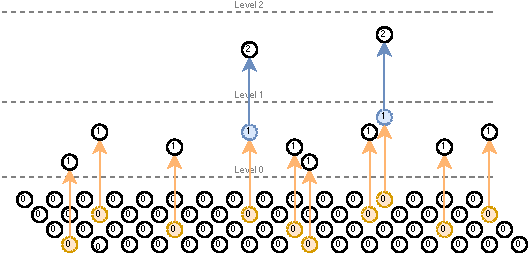
\includegraphics[width=400pt]{figures/Lottery-Standard}
\caption{Sketch of the Lottery process, nodes goes from one level to the next
    with probability $P$} \label{fig:ClusterBunch-Bunch}
\end{figure}

\paragraph{Bunch} A node can compute its bunch in the following manner. It
looks at every other node by order of distances in ascending order and
includes it in its bunch if its level is not smaller than the one it encounters
so far, including its level [\autoref{fig:ClusterBunch-Bunch}]. 

\begin{figure}[!h] 
\centering
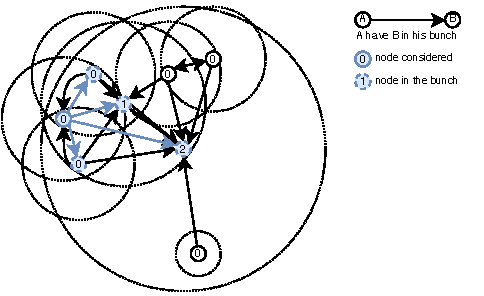
\includegraphics[width=250pt]{figures/ClusterBunch-Bunch}
\caption{ The bunch of the node is depicted in blue. The cluster of the higher
    level node covers the whole system. } \label{fig:ClusterBunch-Bunch}
\end{figure}

\paragraph{Cluster} A cluster is a complementary concept. The cluster of node
$A$ is defined as the set of other nodes that have $A$ in their bunch
[\autoref{fig:ClusterBunch-Cluster}]. 

\begin{figure}[!h] 
\centering
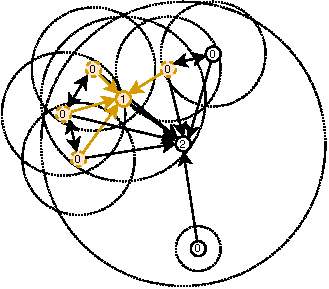
\includegraphics[width=250pt]{figures/ClusterBunch-Cluster}
\caption{ The cluster of the node is depicted in orange. The cluster of the
    higher level node covers the whole system. }
    \label{fig:ClusterBunch-Cluster}
\end{figure}

\begin{figure}[!h] 
\centering
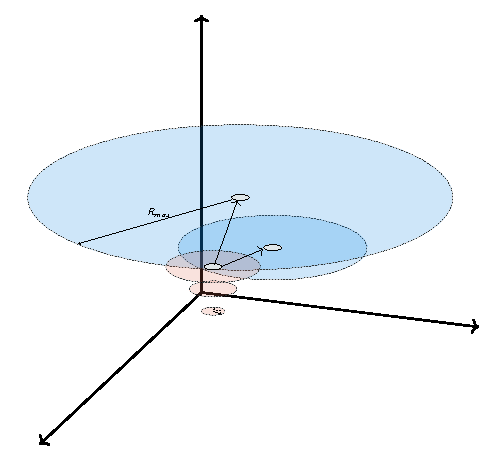
\includegraphics[width=350pt]{figures/regions/ellipsis}
\caption{ A node participates in two kinds of regions. The ones it creates with
    a radius from $R_min$ to one that is covering its cluster (orange). And
    some regions created by the nodes in its cluster, which are covering him
    (blue).} \label{fig:RegionCreation}
\end{figure}

The smallest region radius $R_{min}$ is defined for the whole system. Each node
will construct $ARAs$ around itself starting at $R_{min}$ and doubling the
radius at each time. It stops at the first $ARA$ that is covering its entire
cluster [\autoref{fig:RegionCreation}]. 

By the lottery, most nodes will be level-zero nodes. Therefore their cluster
supposed to be small, conducting to the creation of a small number of $ARA$s.
The small number of nodes that are at level $K-1$ will have every other node
in their cluster by construction. This means that there will be at least one
$ARA$ that covers the whole system. 

%%%% Nyle
% - Problems it solves - Link with CRUX - Environment - Type of Blockchain 
% - What is already implemented 
% - Next steps. 
%%%%%%%%%%%%%%%%%%%%%%%%%%%%%
\section{Nyle - A Locality-Preserving Blockchain}

Nyle is a cryptocurrency that uses locality to answer some classical problems
of blockchains. Two main problems are addressed: WWIII scenarios and approval
time for a transaction.
 
\paragraph{WWIII Scenarios} \label{WWIII} In case of a WWIII, we can expect to
have at least a long-lasting partition that will split the system in two. This
is a problem for classical cryptocurrencies like Bitcoin \cite{Nakamoto2009},
because for a block to be approved, the users are supposed to wait to have a
global consensus. This consensus will not be reached with a long-lasting
partition and therefore it will create problems for classical cryptocurrencies.
Nyle solves this issue by design using locality.

\paragraph{Approval Time for a Transaction} \label{approve_time} Another issue
with waiting global consensus is that it usually takes a long time. If a
customer wants to use a cryptocurrency in daily life, the nodes should be able
to validate (at least partially) transactions relatively fast. The solution
provided by Nyle use locality again: with Nyle, a transaction can be validated
at different geographical levels, and it is up to the customer to wait for a
local, or global validation for a transaction. For small transactions, for
example for buying a coffee, the customer might agree to only have local
validation. For bigger transactions, he might want to wait a bit longer to have
global validation.

\subsection{Description}

Nyle uses \textit{ARAs} as the representation of one region. In each of these
regions, there will be a copy of the same system, in the case of Nyle, the
system is a blockchain. So each region will have its blockchain and validate
all the transactions between the nodes that are included in it. Some nodes can
be included in different regions, and they will send their transactions to all
the regions they are part of. As all nodes participate in the global region by
design, this ensures that a transaction will eventually be seen by all nodes.

The big difference between CRUX \cite{Basescu2014} and Nyle is that the purpose
of CRUX \cite{Basescu2014} is to work in environments where machines are
relatively "stable" which means that they are not supposed to churn, and more,
where the machines are not supposed to move or to join. This is not the case
for Nyle: if we have a cryptocurrency, we can expect to have deficient,
malicious and moving nodes. This will add some difficulties that will be
managed by the protocol.

Each region will have its blockchain. In Nyle, the choice for the blockchain
will be chosen between ByzCoin \cite{Kogias2016} or Omniledger
\cite{Kokoris-Kogias2017}. But it can be generalized to any kind of blockchain.

\subsection{What is already implemented for Nyle} \paragraph{CRUX algorithm for
region creation} We already have an algorithm for drawing regions
\cite{Basescu2014}.

\paragraph{Block storage on node} As each node will participate in different
regions (from very local to worldwide), it will need to store the blockchain
for all of these regions. We have a method that reduces the redundancy, by only
storing the hash of a block instead of the full block at each level
\cite{Sierro2019}. 

\paragraph{Proof-of-Location} We already have a protocol for controlling the
distance from a new node to the rest of the nodes. And that assures no one
cheats by giving false distances \cite{Kall2019}. 


%%%%% Motivation
% - Already have a system working for a non-byzantine no-churn system 
% - Dealing with these problems can be done by dealing with nodes insertion,
      %  deletion and moving.
% - If we solve that then we can return to the previous system and everything
      %  should be working
%%%%%%%%%%%%%%%
\subsection{Purpose of This Project: Motivation for a Control Plane}

CRUX \cite{Basescu2014} proposes a system that is working in a stable system
(with low-churn) and where nodes do not move too much. As this situation
corresponds to some systems like a wide-area database. It is not
the case of a cryptocurrency. For this kind of system, one can expect to have
at least some churn, some moving nodes and some joining nodes. If the
system has a precise protocol for dealing with nodes entering, leaving and
moving in the system, then the problem of the evolution of the system is
solved. Indeed the churn phenomenon can be described as some nodes leaving the
system and optionally reentering later. 

Therefore the purpose of the control plane will be to deal with the evolution
of the regions that follow the evolution of the nodes in the system. Once that
problem is solved, the blockchain can be replicated in the evolving region and
the strategy will be the same as in CRUX \cite{Basescu2014}. This project
introduces a control plane, that is in charge of the evolution of the nodes. In
particular, it will be in charge of dealing with nodes joining, leaving and
moving. The blockchains are replicated in all the regions, but the control
plane will be global. 

%%%%%%%%%%%%%%%%%%%%%%%%%%%%%%%%%%%%%%%%%%%%%%
\chapter{Design} \label{chap:Design} %%%%%%%%%%%%%%%%%%%%%%%%%%%
%%%%%%%%%%%%%%%%%%%%%%%%%%%%%%%%%%%%%%%%%%%%%%

%%%%%%%%% 
% - Problem definition (Hypothesis, Goals, ...) (2-3p) 
%% - Hypothesis on the threat model
% - First version: Simple Control Plane (15-20p ?) 
%% - Graphs: Control flow, Protocol flow trough time 
%% - Tools: Description of each subprotocols 
% %%%(consensus via Blscosi, gossips protocols, ...). 
%%  - Discussion
%%%% - Advantages, prove that it fulfils the goal
%%%%%% - Graph of difference between system without control plane and with. 
%%%% - Drawback (evaluation of computational, memory and communication costs)
%%%%%% - With graphs
%% - Security Analysis 
%%%%% - 2-3 scenarios illustrating malicious behaviours (written and/or with implementation)
%%%%%%%%%%%%%%%%%%%%%%%%%%%%%%%%%%%%%%%%%%%%%%%
This part will describe the design of the Control Plane, which has the mission
to solve the problem of node insertion, deletion and movement inside the
system.

\section{Problem definition}
%%%%%%%%%%%%%% Problem definition
%% Hypothesis : 
%%  - one-to-one communication
%%  - synchrone network
%%  - Correlation between pings and distances
%%  - Nodes are malicious
%%  - Adversary can delay communication
%%%%%%%%%%%%%%%%%%%%%%%%

\subsection{Hypotheses}
Three hypotheses are made on the network. First, it assumes an Internet-like
network with one-to-one communication. Each node can contact any other nodes.
The network is supposed to be synchrone. This means that every message sent by
a node to another will arrive in order and that a message that is sent will be
received within a given window of time. The third hypothesis is made on the
geometry of the network. It states that for small pings (under 100ms) the
round-trip-time is correlated with the distance between two nodes. This is the
case for the Internet network \cite{Seibert2014}. On this result, we build the
locality properties of the system. 


%%%% mostly copied from
% https://docs.google.com/document/d/1xz1jTphKqxxkAucdh_oOqsFXH147Cjlzcnjmt-yx-f8/edit#heading=h.aq4k1vxbt0t0
\section{General Presentation}

The Control Plane is composed of five different components [FIG.
\autoref{fig:modules}], each necessary to solves different part of the problem.
It needs a membership component, to define precisely which nodes are in the
system at any time. It needs a distance oracle which gives the distance between
two nodes in the system. Then it needs a region management component, which
will create and update the regions based on the membership and the locality.
The time will be split into epochs, a component is in charge of dealing that
aspect. And finally, the control plane is in charge of answering some requests
linked to the location and presence of the nodes in the system. Each component
will be described in detail below. 

\begin{figure}[!h]
\centering
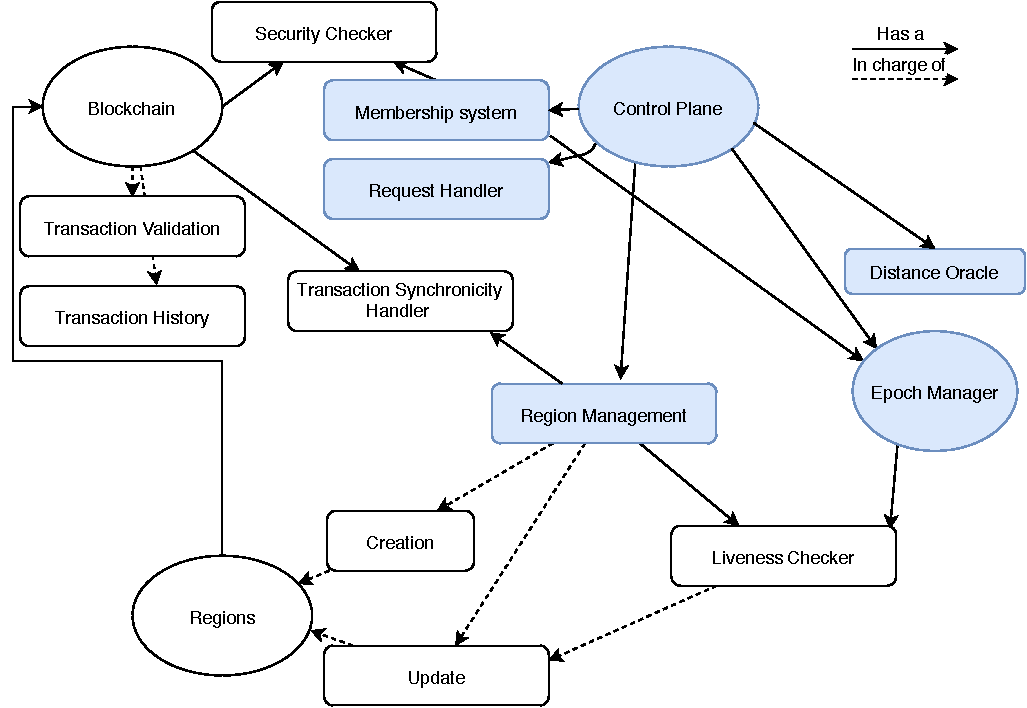
\includegraphics[width=400pt]{figures/Nyle_components}
\caption{List of modules of Nyle. This works concerns the components in blue}.
\label{fig:modules}
\end{figure}

\subsection{Membership Component}

At each epoch, a contract containing a summary of all participants for the
current epoch is created. It is based on registration, which can be made during
the previous epoch. Registration use \textit{endorsement} (for example solution
to a proof-of-work problem). This system will be global. Nodes can ask the
participants of the system to know the identity of other nodes. To validate a
new contract it should be signed by the majority of the nodes of the previous
epoch.

\subsection{Distance Oracle}

The role of the locality component is to give all pairwise distances between
nodes of the system. We assume it already exists (distance oracle), or it can
be computed by nodes. In the first model, the metric that is used as a distance
is latency and all pairwise-latencies are computed between each node and every
node agree on them via consensus. 
 
\subsection{Region Component} This component is used to create and update
regions. This part will be based on CRUX. At each epoch, CRUX is run based on
the new registration, and regions are created.
 
\subsection{Epoch Component} The epoch manager is linked to the membership
system (we allow to change membership at the beginning of one epoch). New nodes
can register during one epoch and join for the next. If nodes have moved, the Region
component will change or maintain their assignment at the beginning of one
epoch. If nodes have crashed, they won't be able to join for the next epoch and
will, therefore, leave the system.

Epochs happen at a defined rhythm (e.g. one day). This frequency can be
shortened to ensure that nodes that want to join do not wait too long, or made
longer if one wants regions not to be redrawn too frequently. 

\subsection{Request Handler} The control plane is the right part to get
requests as it is aware of the nodes location and region assignment. It will be
in charge of answering the request for nodes assignment and nodes location. 

\begin{figure}[!h] 
\centering
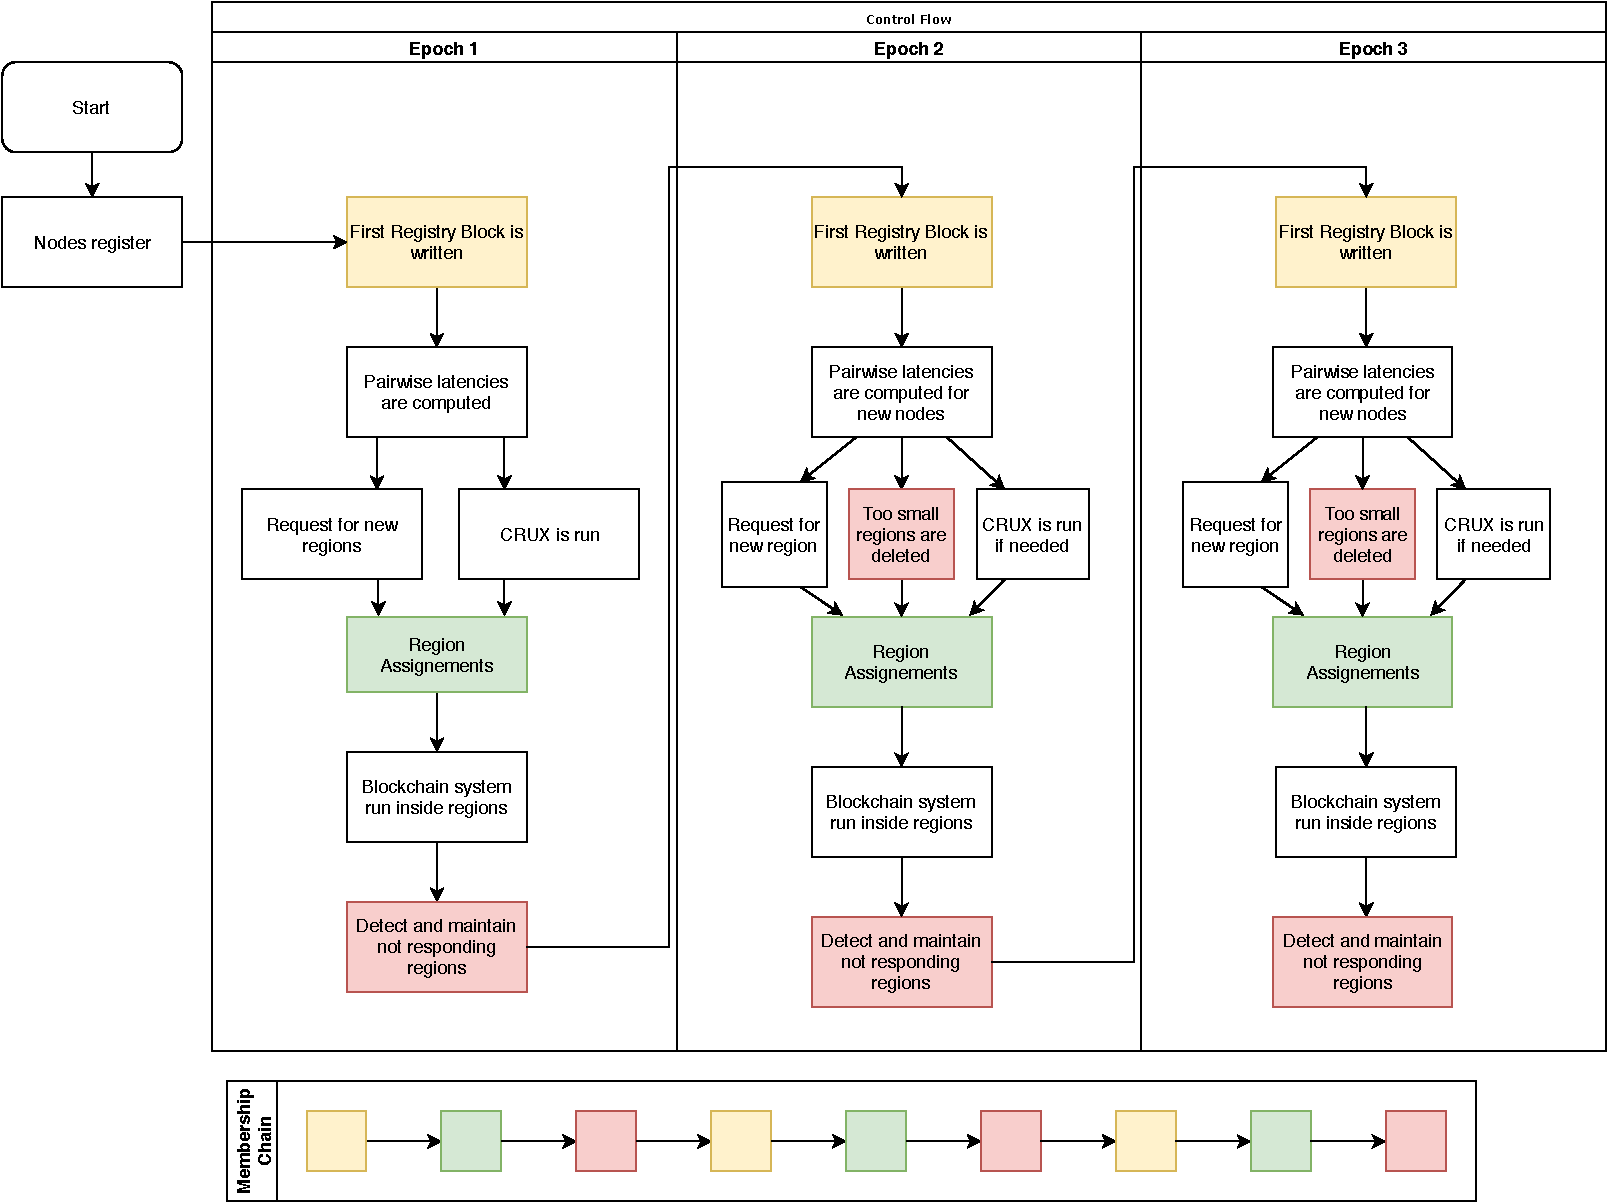
\includegraphics[width=400pt]{figures/Nyle_controlflow}
\caption{General Control Flow of Nyle. }
\label{fig:controlflow}
\end{figure}

\section{Simple Control plane} This version presents the first version of the
Control Plane. In which most of the work is done on the membership component.
At each epoch, nodes can join if they manage to get approval from the members
of the previous epoch. The distance oracle requires a lot of resources: every
node measure pings to every other nodes and consensus is made on that
information. The region component in this model is simple: based on the
registration, and the pings, CRUX is run at each epoch. Redrawing the map of
the entire system. 

\subsection{Membership Protocol}

\begin{sidewaysfigure}[!h]
\centering
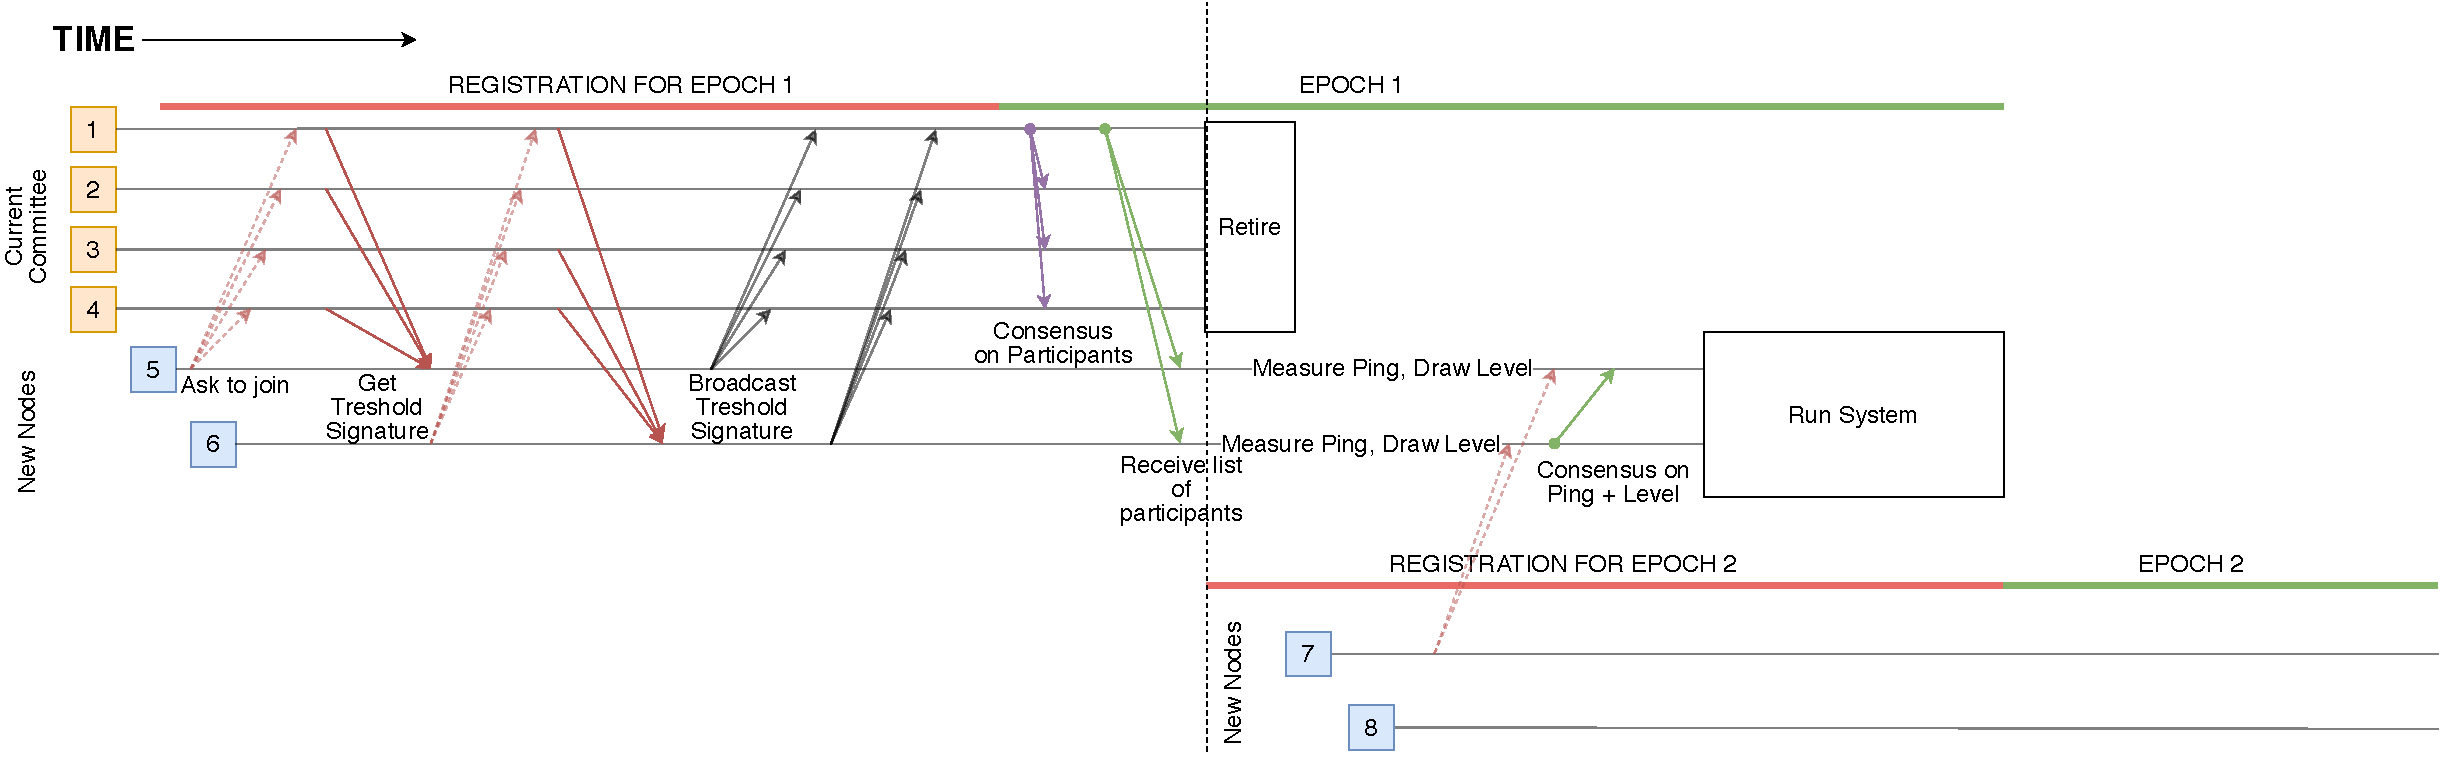
\includegraphics[width=700pt]{figures/Registrationprotocol}
\caption{Sketch of the Protocol.}
\label{fig:registrationprotocol}
\end{sidewaysfigure}

This section describes the membership protocol [\autoref{fig:registrationprotocol}].
The system will go through some cycles (called an epoch) of two different phases :
the registration period and the live period. The first period is there
to manage the participants of the current epoch, and the underlying system
(e.q. a cruxified-blockchain) will be run during the live period. Assume
that each node has a synchronised wall-clock which gives the time of the
different periods.

The authority that will decide which node participates in the next epochs is
the participants of the current epoch, which will be called the \textit{admission
committee}. Assume that a set of genesis participants, which will be the first
 \textit{admission committee}, exists.

\paragraph{Registration Period}
If a node wants to register for the next epoch, it has to send the following
information to the admission committee : a \textit{name}, a \textit{public key}, and an
 \textit{endorsement} (for example solution to a proof-of-work problem) and ask for a
 \textit{threshold-signature}. 

If the new node manages to get back a threshold-signature from the admission
committee, it has to broadcast it again to the admission committee during the
same registration period. The current committee will then acknowledge that it
is a participant for the next epoch. This is necessary as nodes in the
committee might not necessarily know if the admission they signed managed to
reach the threshold. The admission committee will aggregate the
threshold-signatures for all the participants for the next epoch. At the end of
the registration period, the admission committee will reach a consensus on the
new participants, by threshold-signing the list of the members.  

\paragraph{Live Period}
At the beginning of the live period, one member of the admission committee will
send the threshold-signed contract that lists the participants to the current
members. If one of the participants did not receive the list, it can ask any
member of the admission committee to have it. After that propagation, the
admission committee can retire, and the member of the current epoch becomes the
new admission committee. Then members of the new epoch will compute the
distances between each other. Participants will as well draw a level from
unpredictable, bias-resistant public randomness source. They will then reach
consensus on those ping-distances and levels by threshold-signing them and
broadcast them.  At this point, each member of the new epoch will have the same
view of the system as they will know the participants, the latencies between
each one of them and their levels. Therefore these participants will be capable
of running the system in a deterministic manner.

Following the election of the new admission committee at the beginning of the
live-epoch, the registration period for the next epoch can begin, as the
authority that will accept admission is running. Registration period and live
period can, therefore, be superposed [\autoref{fig:registrationprotocol}], which
permits to have a system running at every time. 

\subsection{Threshold-Signing Admission}
To get an admission a node that wants to join for the next system will use the
BlsCoSi protocol \cite{Boneh2018}. It will generate a tree with him as
the root and the admission committee as nodes in the tree. Each node of the
admission committee will have the choice of signing or rejecting the admission
request. The threshold will be set at the majority. So if a node manages to get a
majority of signatures then it will be accepted in the system. A node from the
admission committee is supposed to accept the query if it has not already seen
the node, and if the \textit{endorsement} is convincing and was made with the public-key
associated. This ensures that a node cannot steal the endorsement of another
for registration.  

\subsection{Committee Consensus}
Committee consensus is used at two different times. First at the end of the
registration period. Consensus should be reached by the admission committee to agree on
the participants of the next epoch. A random member of the admission committee
is selected to run the consensus protocol. It will send the list of members
that it aggregated during the registration period. And try to get a threshold
signature on it from the other member of the admission committee. Members of
the admission committee are supposed to sign the list if they aggregated the
same list of members for the next epoch.

If one member does not manage to reach consensus, another can be selected to
run the consensus. A communication round can be added between two consensus
phases so that every member of the admission committee broadcast its list
of members with valid proofs.

The same idea is used at the beginning of the live epoch to reach consensus on
the list of pings between every member of the system and on the levels on all
nodes in the system.
% TODO: think about what to do if the consensus is not manageable. 

\subsection{Public distributed source of randomness}
To draw the levels for the region creation algorithm, a distributed public
source of randomness will be used. This can be targeted by adversaries trying
to get a specific level which can unbalance the system, as described in
\autoref{app:unbalanced-levels}. To be sure that this source is not targeted,
it is based on the information created during the consensus on the participants
just before drawing the regions. 

\FloatBarrier
\section{Discussion}
\subsection{Advantages}
This simple version of the control plane is solving the problem of node
insertion, churn and nodes movement in the system. A comparison will be made
with a fixed version only using CRUX for region management but without a
control plane. The the system begins with a fixed number of nodes and creates
regions based on CRUX, then the system is replicated inside all regions, with
no update possible.

\subsubsection{Nodes Insertion}
The version without a control plane cannot add nodes to the system. Indeed a
fixed number of nodes is required to create the regions. With this control
plane, node insertion is possible at the beginning of every epoch
[\autoref{fig:insertion-comparision}].

\begin{figure}[!h] 
\centering
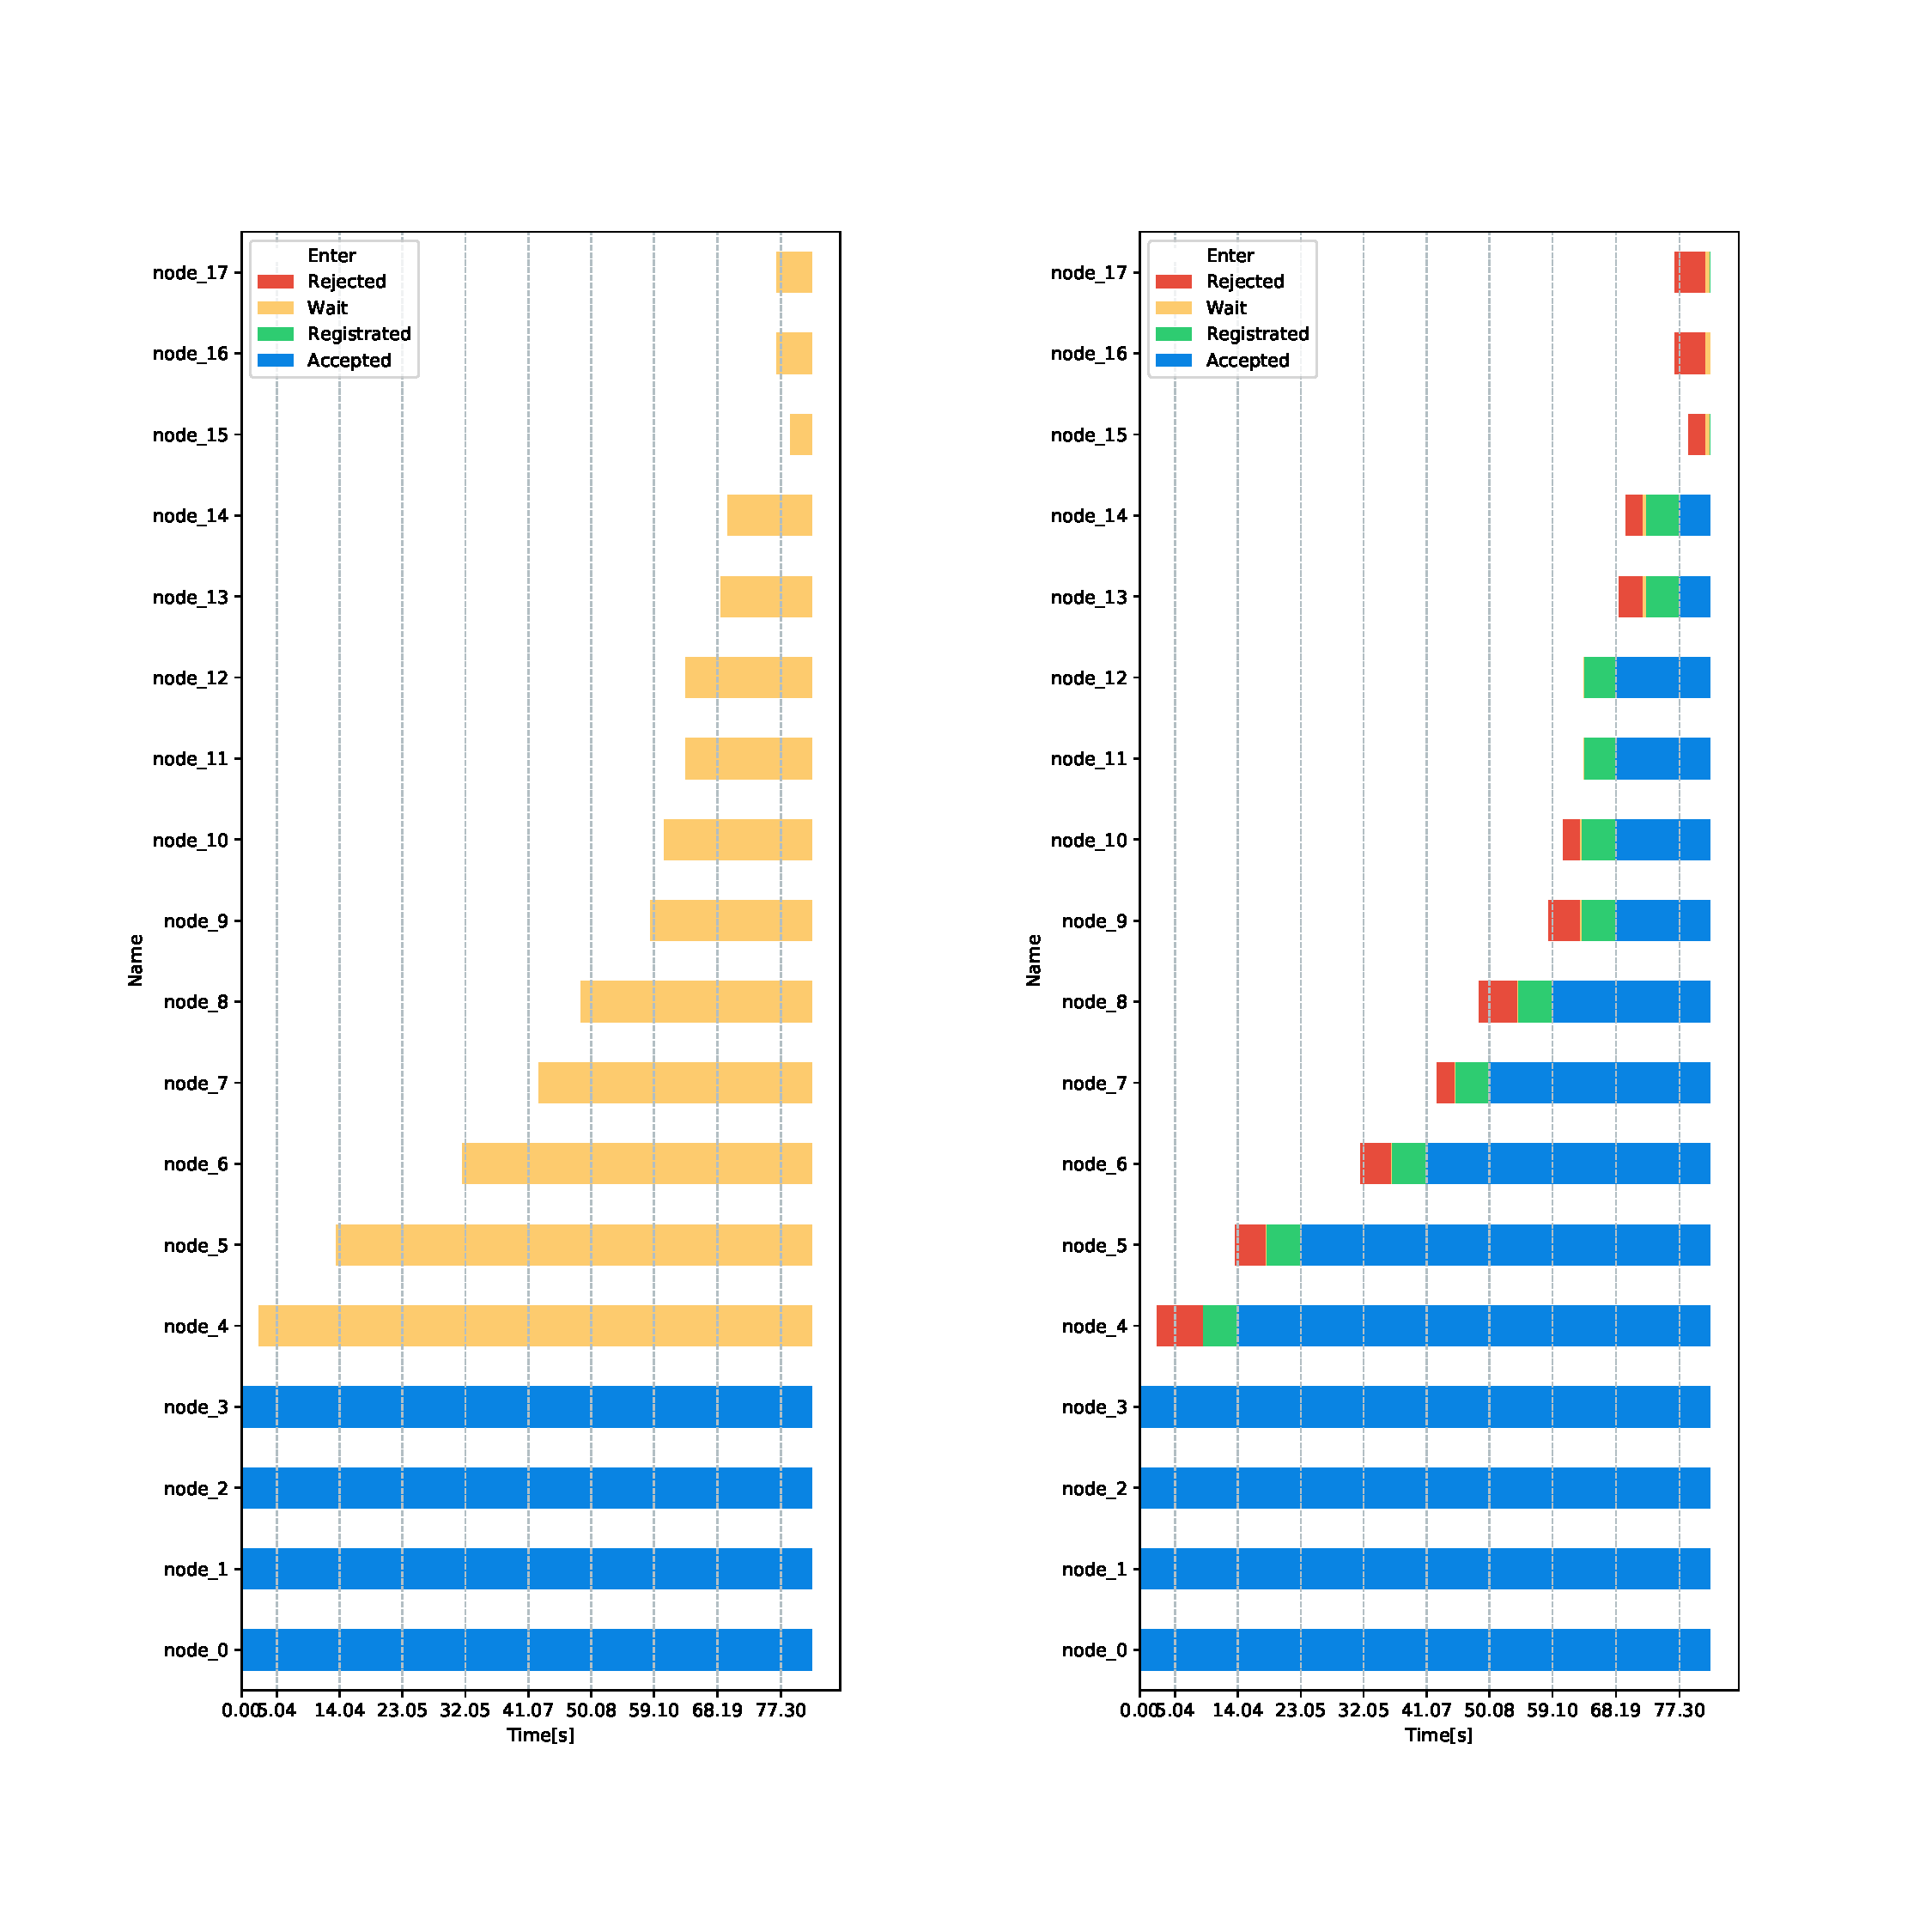
\includegraphics[width=450pt]{figures/JoinSubplots}
\caption{The simple control plane allows nodes to join the system. The left plot
  represents the case with a fixed control plane where nodes cannot join. The ticks are placed at the start of epochs. }
  \label{fig:insertion-comparision}
\end{figure}

\subsubsection{Churn Resistance}
Nodes can churn. If the system is not supposed to change, crashing nodes can still be
in the system. With this control plane, nodes that have crashed cannot
register for the next epoch and therefore are removed from the system [\autoref{fig:churn-comparision}]. 

\begin{figure}[!h] 
\centering
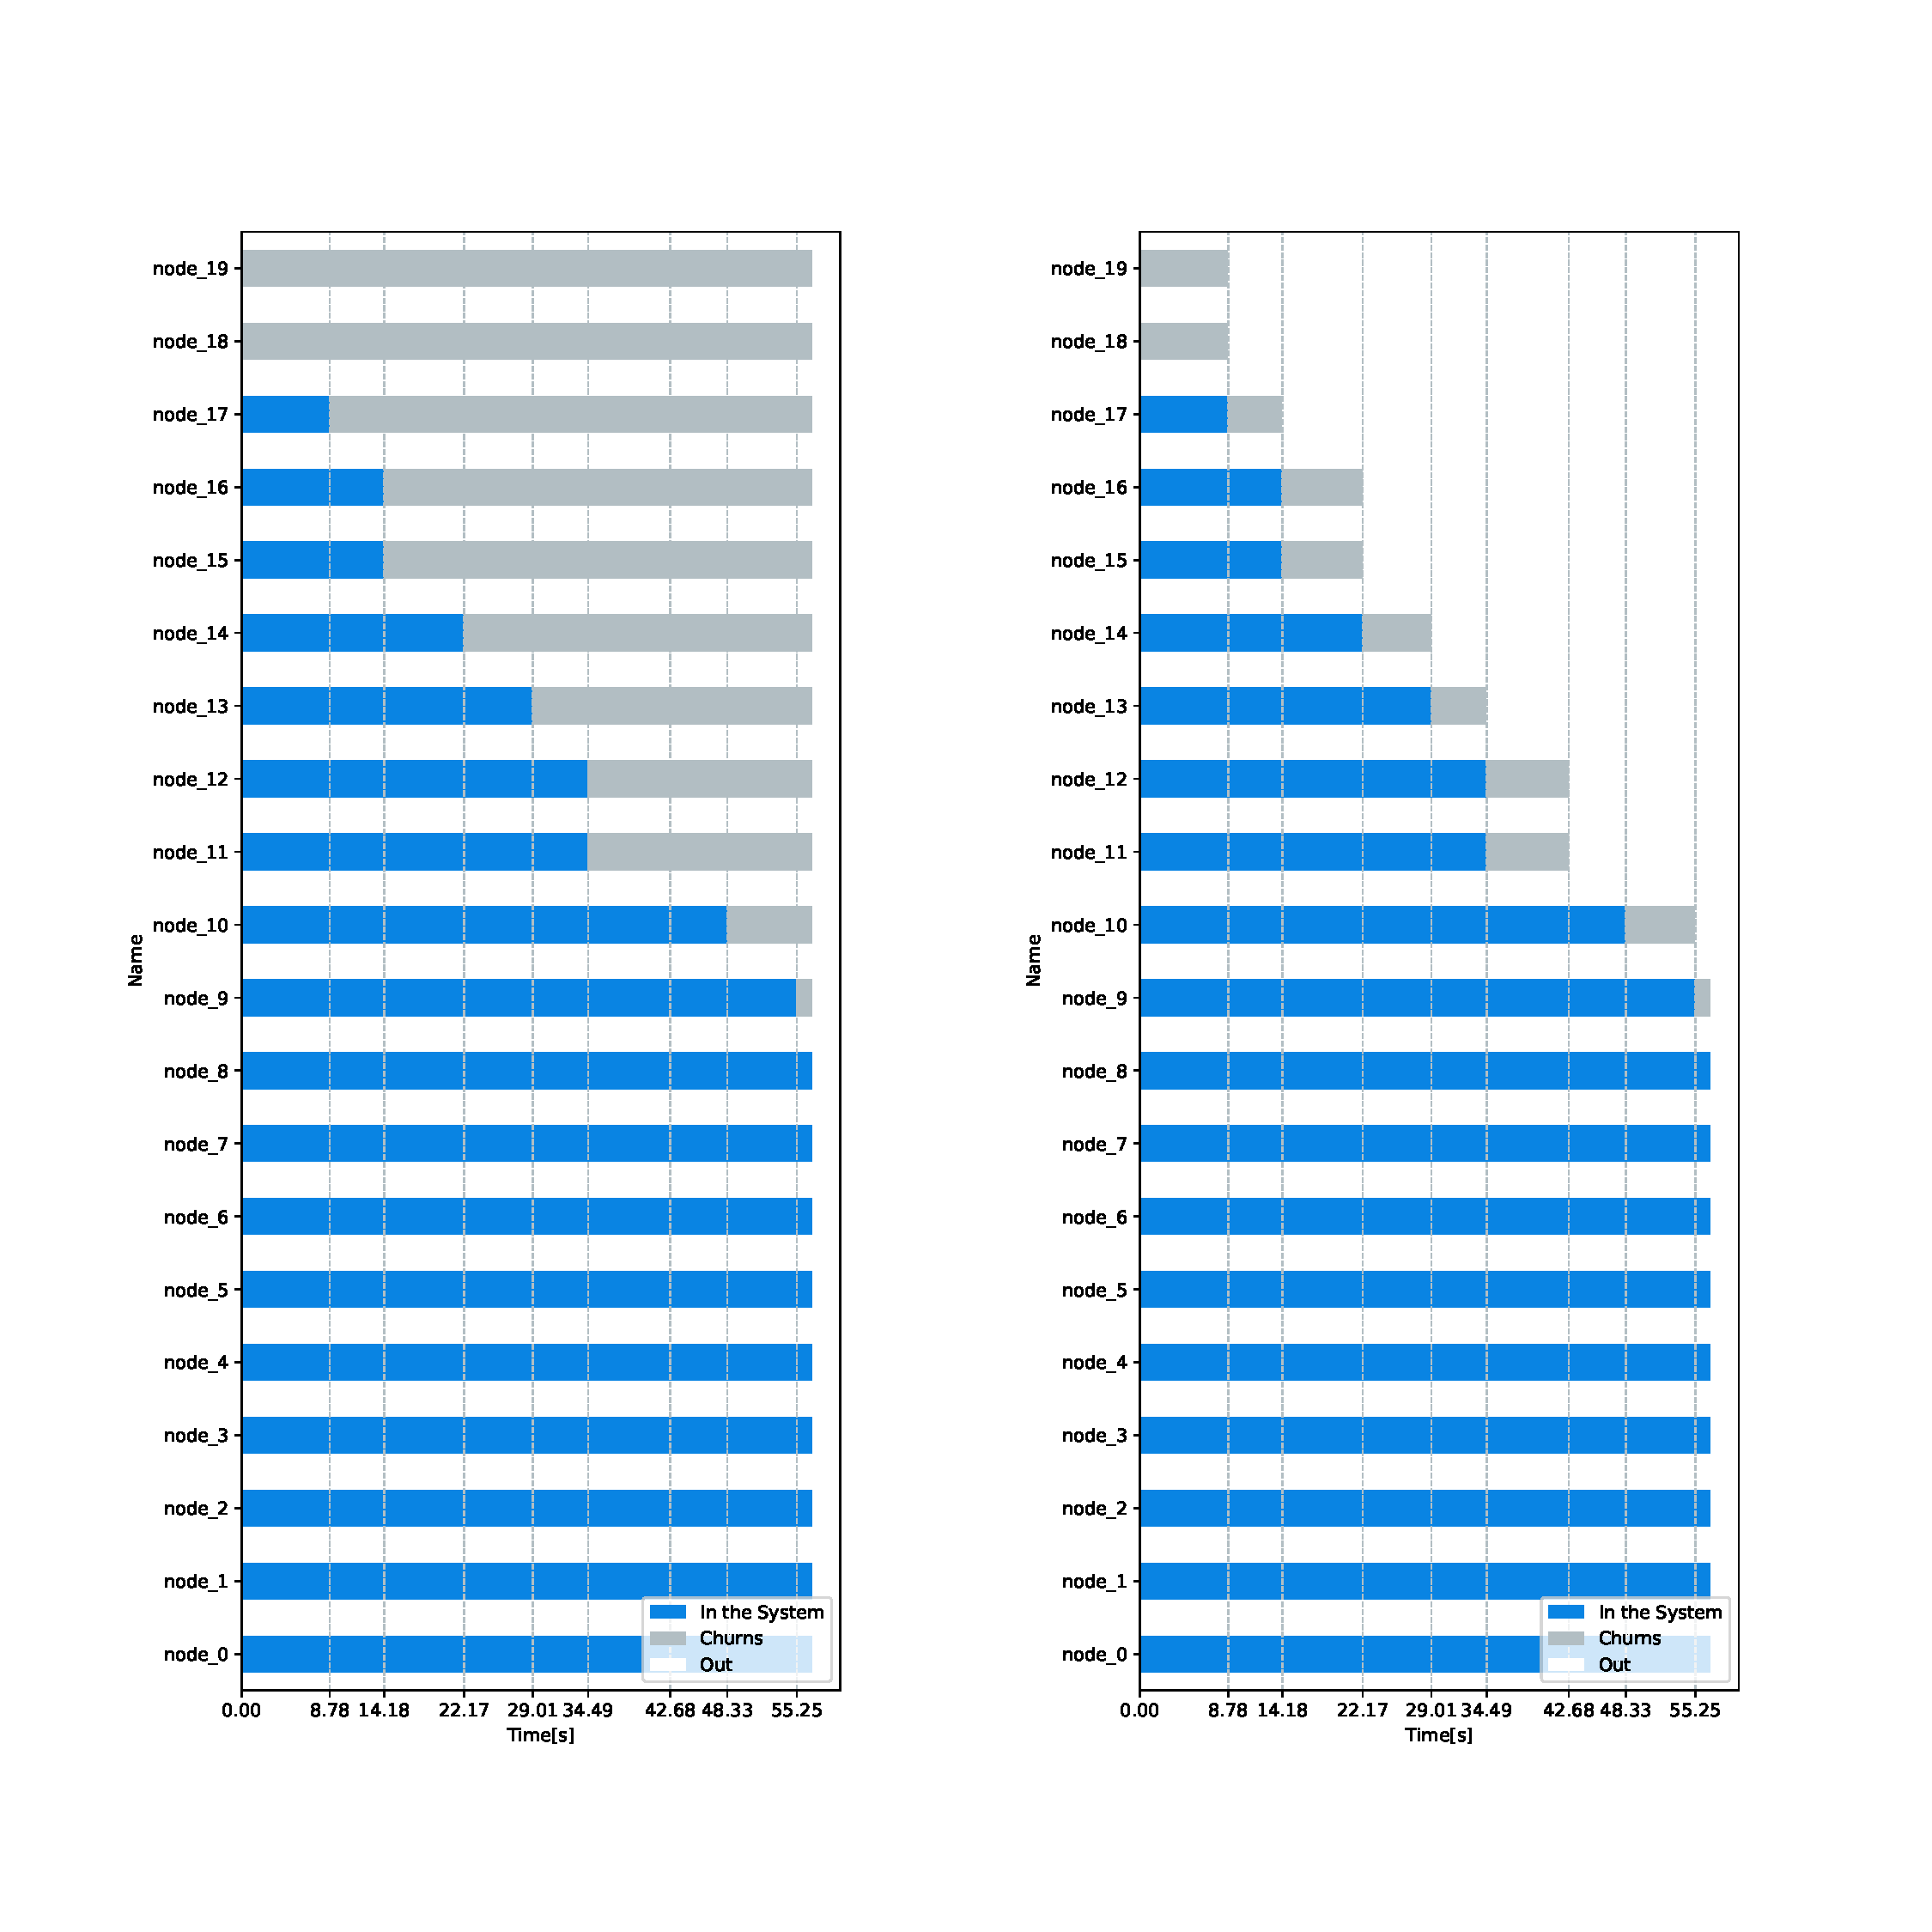
\includegraphics[width=450pt]{figures/ChurnSubplots}
\caption{The simple control plane remove nodes that have left the system. The
  the left plot represents the case with a fixed control plane where nodes cannot leave. The ticks are placed at the start of epochs.}
  \label{fig:churn-comparision}
\end{figure}

\subsubsection{Adaptation to Node Movements}
Nodes can move as well if the regions are only drawn at the beginning of the
system. Then it's possible that after a while a lot of nodes have migrated from
where they were at the time that the regions were drawn. This might be a
problem, indeed, the purpose of the replication was to ensure that in case of a
partition, nodes participating in the same side of the partition should still
be able to work. If most of the nodes have moved, but are still participating
in the region of their first assignment, a partition could happen somewhere in
the system leading to failing regions that should be on the same side of the
partition. The control plane solves this problem as the regions are recreated at
each epoch taking account of the movement of the nodes. Increasing the
partition resistance, with the movement of nodes.

\subsection{Drawbacks}
This control plane is simple and reaches its objective, but it requires a lot of
resources. Some of the drawbacks of this approach are listed below. 
Some answers to these drawbacks are proposed in \autoref{chap:Improvements}.  

\subsubsection{Control Plane is global}
If the system is replicated in all the regions, the control plane itself is
global. Meaning it could be subject to a partition. In this case, the replicated
system would continue to work, but the control plane could only continue to
work on the side of the majority. This is not a major drawback as the main
purpose, the continuity of the underlying system is guaranteed. However, the
evolution of the system in the side of the minority will not be treated by the
control plane.

\subsubsection{Epoch Transition Requires Resources}
Epoch transition requires a lot of resources, indeed first it needs a lot of
communication for the consensus and the registration as every node that was
previously on the system should be contacted by every new node. If $\bar{N}$ is
the average number of participants in epochs. Then registration 
requires $O(\bar{N}^2)$ messages. As every new node has to send a message
to every member of the previous committee. This can be inefficient. 

Then when the registration is done, the protocol as it is will redraw most of
the regions as the algorithm for region creation is reused. This can be
inefficient as well because some transfer of information between old regions
and the new one might be expected.

%% TODO FIT
\begin{figure}[!h] 
\centering
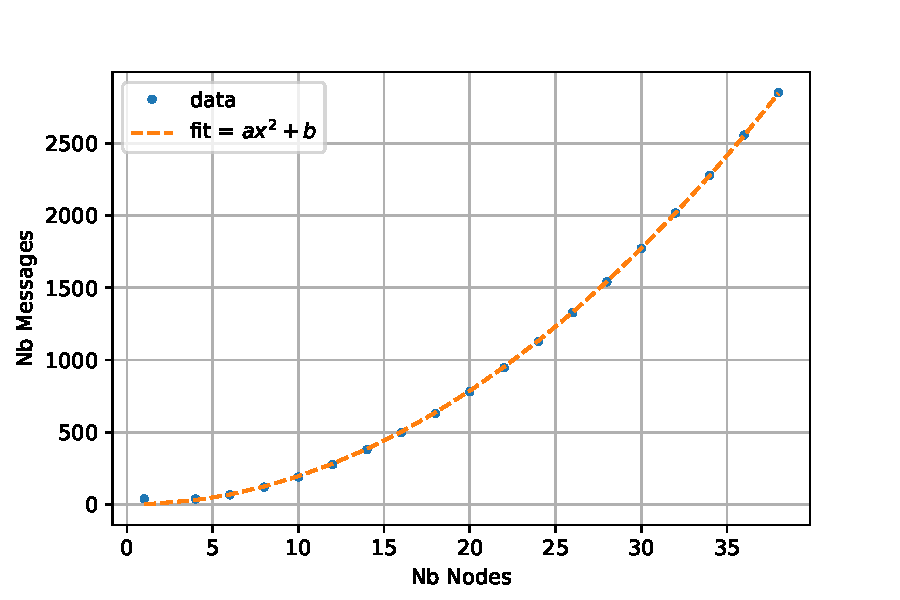
\includegraphics[width=350pt]{figures/messages-plot}
\caption{Growth of the number of messages for one epoch with the number of nodes. \color{red} TODO FIT \color{black}}
\label{fig:messages-plot}
\end{figure}

%% TODO FIT
\begin{figure}[!h] 
\centering
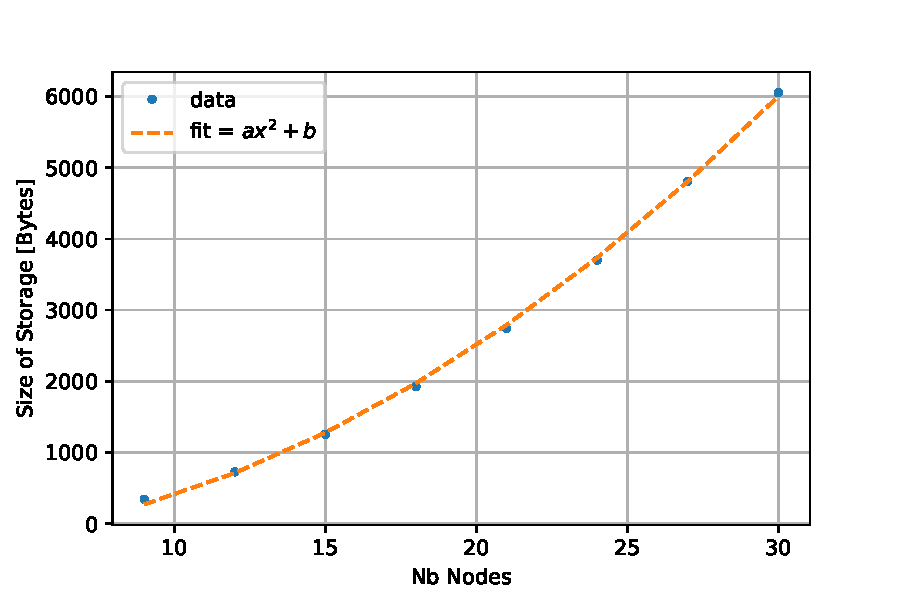
\includegraphics[width=350pt]{figures/storage-plot}
\caption{Growth of the amount of storage required for ping distances for one epoch with
  respect to the number of nodes. \color{red} TODO FIT \color{black} } \label{fig:storage-plot}
\end{figure}

 
\subsubsection{Omniscience of the Nodes}
Nodes are aware of a lot of information. By design, they are aware of
the list of every other node in the system, their levels, the pings between
each pair of nodes in the system, all the region created and all the region
assignment. The nodes need to be aware of this information so that
every node will run the algorithm for region creation and arrives in the same
regions. But this can be a lot of information to store.

\section{Security Analysis}

\subsection{Threat Model}
Attacks on the system can be made internally (from malicious nodes) or
externally by delaying the interaction between nodes or intercepting and
changing messages. We will give the precise portion of malicious nodes that
this protocol can handle. In this threat model, malicious nodes are regular
nodes that decide to act against the system. In particular, malicious nodes
have only access to a bounded computational power, and they cannot break the
cryptographic primitives. 

\subsection{Network Attacks} 
\subsubsection{Man-in-the-middle attacks} \label{MitM}
The messages exchanged during the protocol are listed in the following table [\autoref{tab:messages-table}].

\begin{table}[]
\centering
\begin{tabular}{m{0.05\textwidth}m{0.25\textwidth}*{2}{>{\arraybackslash}m{0.3\textwidth}}}
\toprule
&\textbf{Message}                                              & \textbf{Signature}                      & \textbf{Effects of a Sufficient Delay} \\ \midrule
$1.$ & Join request                                                & Requesting node                      & Request refused        \\ \hdashline
$2.$ &Threshold signature of the request                               & Threshold number of the current committee & Request refused        \\ \hdashline
$3.$ &Broadcasting of the Threshold signature                          & Threshold number of the current committee & Request refused        \\ \hdashline
$4.$ &Messages for the consensus on the participants,
list of the participants                                            & Leader of the current committee          & View Change          \\ \hdashline
$5.$ &List of pings and levels                                        & Leader of the current committee          & View Change \\
\midrule
\bottomrule
\end{tabular}
\caption{List of the messages exchanged during the protocol. The signature of the message and the effects of a delay are given. }
\label{tab:messages-table}
\end{table}

As all the messages are signed, if a message is changed, it will be noticed by
the receiver. Which will discard the altered message, and ask again to the
sender. Therefore the only effect of a Man-in-the-middle attack will be to
delete some of the messages, which can be seen as a sort of delay attacks. 

\subsubsection{Delay Attacks}
This protocol is not resistant to delay attacks. It assumes wall-clock
synchronicity between the nodes, which can cause some problems. The effects of
delaying messages are listed in [\autoref{tab:messages-table}]. During the
registration, if the messages are delayed until the start of the next epoch,
then it will lead to the refusal of the request, and the node has to create a
new request for the next epoch. If the messages of the leader of the consensus
for the participants of the pings and levels are deleted or delayed, the other
nodes will ask for a view change: asking the next node in the list to start the
consensus again. If attackers manage to always delay the messages of the
successive leaders, it can block the protocol forever.

\subsection{Malicious Nodes}
\subsubsection{Attack on Consensus} If a malicious
node is already in the committee, the only misbehaviour that it
can do the period is to refuse to sign some messages. Sending forged messages
are already treated in \autoref{MitM} as they are not possible to forge because
of the signature. Refusing to sign join requests can lead to a failing protocol
if the number of malicious nodes is bigger than the threshold required to get
the signature. As the signature procedure is done using BlsCoSi \cite{Boneh2018},
the registration process is subject to the same threat. BlsCoSi
\cite{Boneh2018} is an efficient way to implement The \textit{Practical
Byzantine Fault Tolerance} (PBFT) \cite{Castro1999} algorithm which guarantees
\textit{safety} and \textit{liveness} if the system as no more than $f$ faults
among $N = 3f+1$ nodes.Therefore it is required to have no more than $f$
malicious nodes. As the number of nodes in the system evolves
with time, it required not to have more than this fraction of malicious nodes
in the system at any epoch. If for one epoch, the number of malicious nodes is
bigger, then they can block all the consensus, leading to a failing system. 
If a malicious node is elected as a leader of the consensus on the list of
participants or the pings, it can decide not to start the consensus. After a
while, another node will be elected to run the consensus, which will eventually
succeed if the number of malicious nodes is low enough.

\subsubsection{Attack on Levels} \label{sec:ControlePlane-Threat-Model}
At the beginning of one epoch, nodes compute their bunch and cluster based on
the pings and the levels that are drawn from a shared public source of
randomness which is renewed at each epoch. Nodes deploy region covering its
cluster. Each node will participate in regions along its bunch. It is important
to realize that this procedure is not based on the action of a node, but just
on the fact that they exist at a given place and a given level. What is meant
by that is that every node has the same view of the system. And if node $A$
have node $B$ in its bunch, then node $A$ is supposed to participate in a
region which is based on the position of $B$ and spans the cluster of $B$, but
$A$ already has all the information to know about this region using only the
pings and levels. Therefore node $B$ cannot use a high level to perform an
action that will block the system. 

However, if a malicious attacker could take over the lottery process, it could
manage to group the high level in a side of the system. Leaving only the
level-zero. This could lead to some problem which is described in \autoref{app:levels-zero}.
Taking over the lottery process should not be possible by design. Indeed, the
lottery is based on a public source of randomness that renewed at each epoch
and revealed after the registration of the levels. Nodes can know the level of
other nodes because they base the compute of their levels on the
threshold-signed list they received from the previous committee. The source
must be revealed after registration of the levels, otherwise, malicious nodes
could try to influence the order of the list on which the lottery process is
based. 

%%%%%%%%%%%%%%%%%%%%%%%%%%%%%%%%%%%%%%%%%%%%%%
\chapter{Improvements} \label{chap:Improvements} %%%%%%%%%%%%%%%%%%%%
%%%%%%%%%%%%%%%%%%%%%%%%%%%%%%%%%%%%%%%%%%%%%%

This section proposes some improvements to the simple control plane protocol. They
are supposed to address the drawbacks of the simple protocol, each improvement
will be illustrated in a Strawman model. Finally, an advanced
version of the control plane that uses a region creation algorithm based on
time/space graphs will be proposed. 

\section{Strawman 1 : Locarno Treaties} \label{Locarno}

\begin{figure}[!h] 
\centering
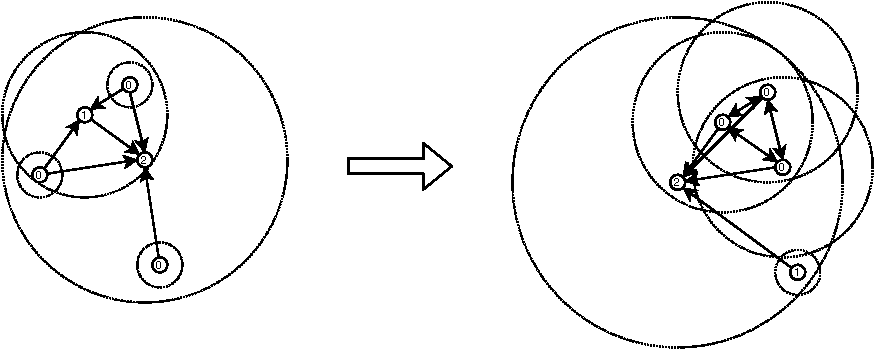
\includegraphics[width=300pt]{figures/LocarnoTreaties-Redrawing}
\caption{Redrawing the levels at each epoch can lead to very different version
  of the system. This is what is improved by the Locarno Treaties. Shrinking
  regions are depicted in red, growing regions in green and same region in
  black.} \label{fig:LocarnoTreaties-Redrawing}
\end{figure}

Following the First World War, it was decided that the borders of Germany
should remain fixed. The Locarno Treaties defined some of these borders. The
idea of this Strawman model is to do the same by limiting modifications of
regions from one epoch to the next. The idea is to use a deterministic set of
rules, based on the ping, the registrations and the map of the previous epoch
to create the map of the current epoch using the fewer modifications possible.
Registration is still global and each node will have all the information about
the memberships of every node. Then from one epoch to another, the purpose of
the game is to keep as many regions as possible. The obvious idea to reach this
goal is to let the nodes keep their levels from one epoch to the next. However,
some small difference should be introduced to avoid some problems.
These are described in the next section.

\subsection{Rebalancing the Levels} \label{rebalancing}
Conserving the levels is the way to go, but maintaining levels can lead to
unequilibred systems. Consider a system with 200 Nodes at epoch 1, with the
repartition given in \autoref{example-lottery}. If from epoch 1 to epoch 2,
100 level-0 nodes leave the system, the remaining system would contain 80
level-0 nodes instead of 90. 

Unbalanced systems can lead to some problems, some examples are given in
\autoref{app:unbalanced-levels}. The lottery process presented in
\autoref{sec:common-tools}, is a bit changed in this part to allow the
adaptation of the levels. The total number of participants $N$ in the system is
known after the registration, and as the probability $P$ is given, it is
straightforward to compute the expected number of nodes that one should have at
every level as it mentioned in \autoref{example-lottery}. 

Instead of drawing the levels directly from a randomness source, nodes will
draw a random number from this source between 0 and 1
[\autoref{fig:sketch-new-levels}]. All nodes can deduce what number the others
will draw deterministically from the registration list and the public source of
randomness. The highest level will go to the node which has drawn the highest
random number. And levels are given according to the drawing in descending
order. Each node that stays in the system will keep its random number from when
it joined the system, new nodes get new random numbers. 

\begin{figure}[!h] 
\centering
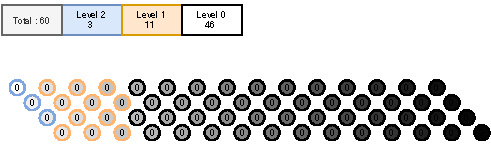
\includegraphics[width=400pt]{figures/Lottery-Locarno}
\caption{Sketch of the new method for drawing the levels. The fill property of each node represents
  the number that was drawn from 0 (black) to 1 (white).}
  \label{fig:sketch-new-levels}
\end{figure}


\subsection{Motivation for Keeping the Levels} This section describes the
reasons for keeping the levels. To understand what are the effects on the
global system it is useful to look in detail at what are the consequences of
the movement of a given node on a given fixed node. Then some precise examples
of the evolution of the system are treated as well. 

\subsubsection{Effects for a Fixed Node} The point of view of one node that
stays fixed in the system is taken, the goal is that the node can keep most of
its region assignments. Other nodes might join, leave or move and this can lead
either to change in its cluster of in its bunch. But additional effects can
come from the level rebalancing
[\autoref{fig:LocarnoTreaties-Leaving-cluster}]. 

\paragraph{Nodes Leaving the Cluster} This can shrink the cluster of the fixed
node. As the regions created by a given node stops when the radius covers the
whole cluster, this might lead to the deletion of some regions. This does not
change the region assignment and the nodes can still keep the replicated system
of the previous epoch running. But additional effects can come from the level
rebalancing. 

\paragraph{Nodes Joining the Cluster} On the contrary, if nodes join the
cluster of the fixed node, this might lead to the creation of an additional
region to cover these extra nodes. The node will then replicate its system to
the newly created regions. But most of the regions are kept the same.

\paragraph{Nodes Leaving the Bunch} Nodes participate in all the region in
their bunch, eventually, they will participate in a region that covers the
whole system. If a node left the system in the bunch, this leads to a region
centred around a point that is not in the system anymore, this assignment might
be forgotten. 

From a fixed node, if another node leaves its bunch, it can have as effect to
add other nodes in its bunch, leading to more region assignment.  And in some
cases, to more nodes in its cluster, leading to region growth. 

\begin{figure}[!h] \centering
    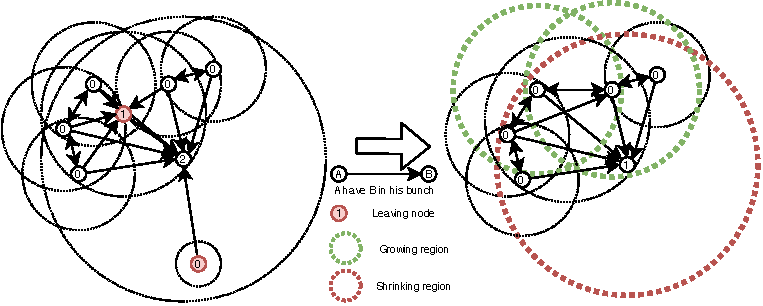
\includegraphics[width=300pt]{figures/LocarnoTreaties-Leaving-cluster}
    \caption{A leaving node is changing assignments of other nodes but keep the
    same regions. Shrinking regions are depicted in red, growing regions in
    green and same region in black. }
\label{fig:LocarnoTreaties-Leaving-cluster} \end{figure}

\paragraph{Nodes joining the Bunch} If nodes are joining in a bunch, this leads
to additional region assignment. 

\subsubsection{Rules for other nodes} The point of view of a fixed node in the
system was treated. Now it stays to look at the case of other nodes. The
question is how to integrate moving or joining in the system while keeping the
system balanced. 

\paragraph{High-Level Moving Node} Assume that going from Epoch $i$ to $i+1$,
one of a relatively high-level node has gone from one place to the other end of
the system. As nodes can keep their level, it will change some of the
assignments, but most of the regions will be maintained. 

\begin{figure}[!h] 
\centering
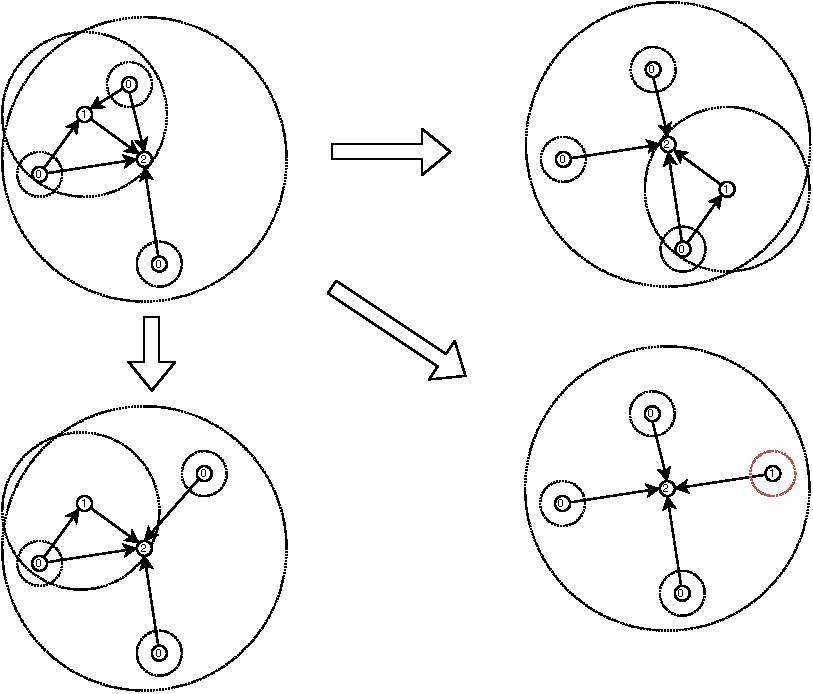
\includegraphics[width=300pt]{figures/LocarnoTreaties-Moving}
\caption{A moving high-level node keeping its levels is changing assignments of other
  nodes but keep the same regions. Shrinking regions are depicted in red,
  growing regions in green and same region in black. }
\label{fig:LocarnoTreaties-Moving}
\end{figure}

This seems to indicate that movement should not be a problem. There is a
slight difference between that situation and changing the levels at each
epoch. As each node can keep its copy of the underlying system working in its
region. If the levels are changed, communication might be needed to transfer
data from one region to another. This communication overhead is reduced in
that situation. 

\paragraph{Levels of Joining Nodes}
One can think that the levels of joining nodes might have a big influence on the
system, this part tries to illustrate what might happen. The joining nodes can
lead to the growth of one region or the creation
of regions. Effects of the level of joining nodes are illustrated in
[\autoref{fig:LocarnoTreaties-Insertion-close}][\autoref{fig:LocarnoTreaties-Insertion-close}].

\begin{figure}[!h] 
\centering
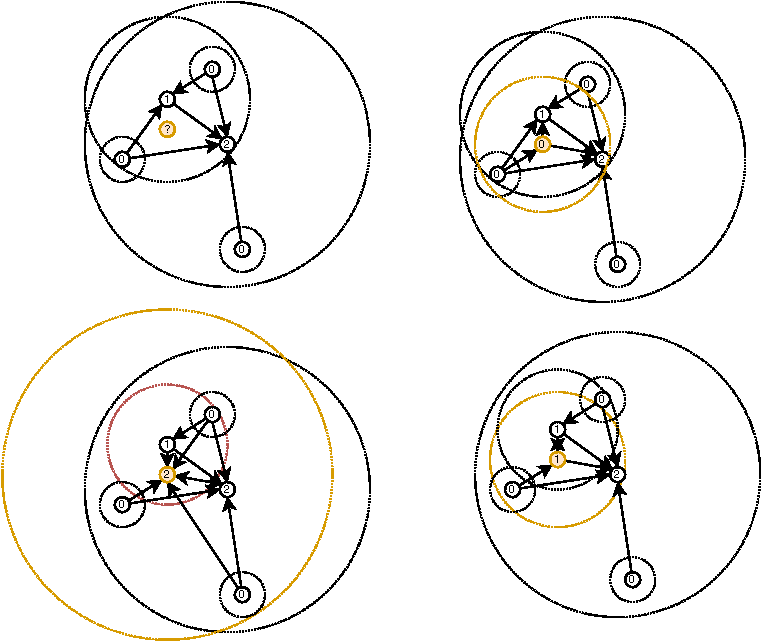
\includegraphics[width=300pt]{figures/LocarnoTreaties-Insertion-close}
\caption{Keeping the same level leads to smaller changes when a node enter the
  system. Shrinking regions are depicted in red, growing regions in green and
  same region in black.} \label{fig:LocarnoTreaties-Insertion-close}
\end{figure}

\begin{figure}[!h] 
\centering
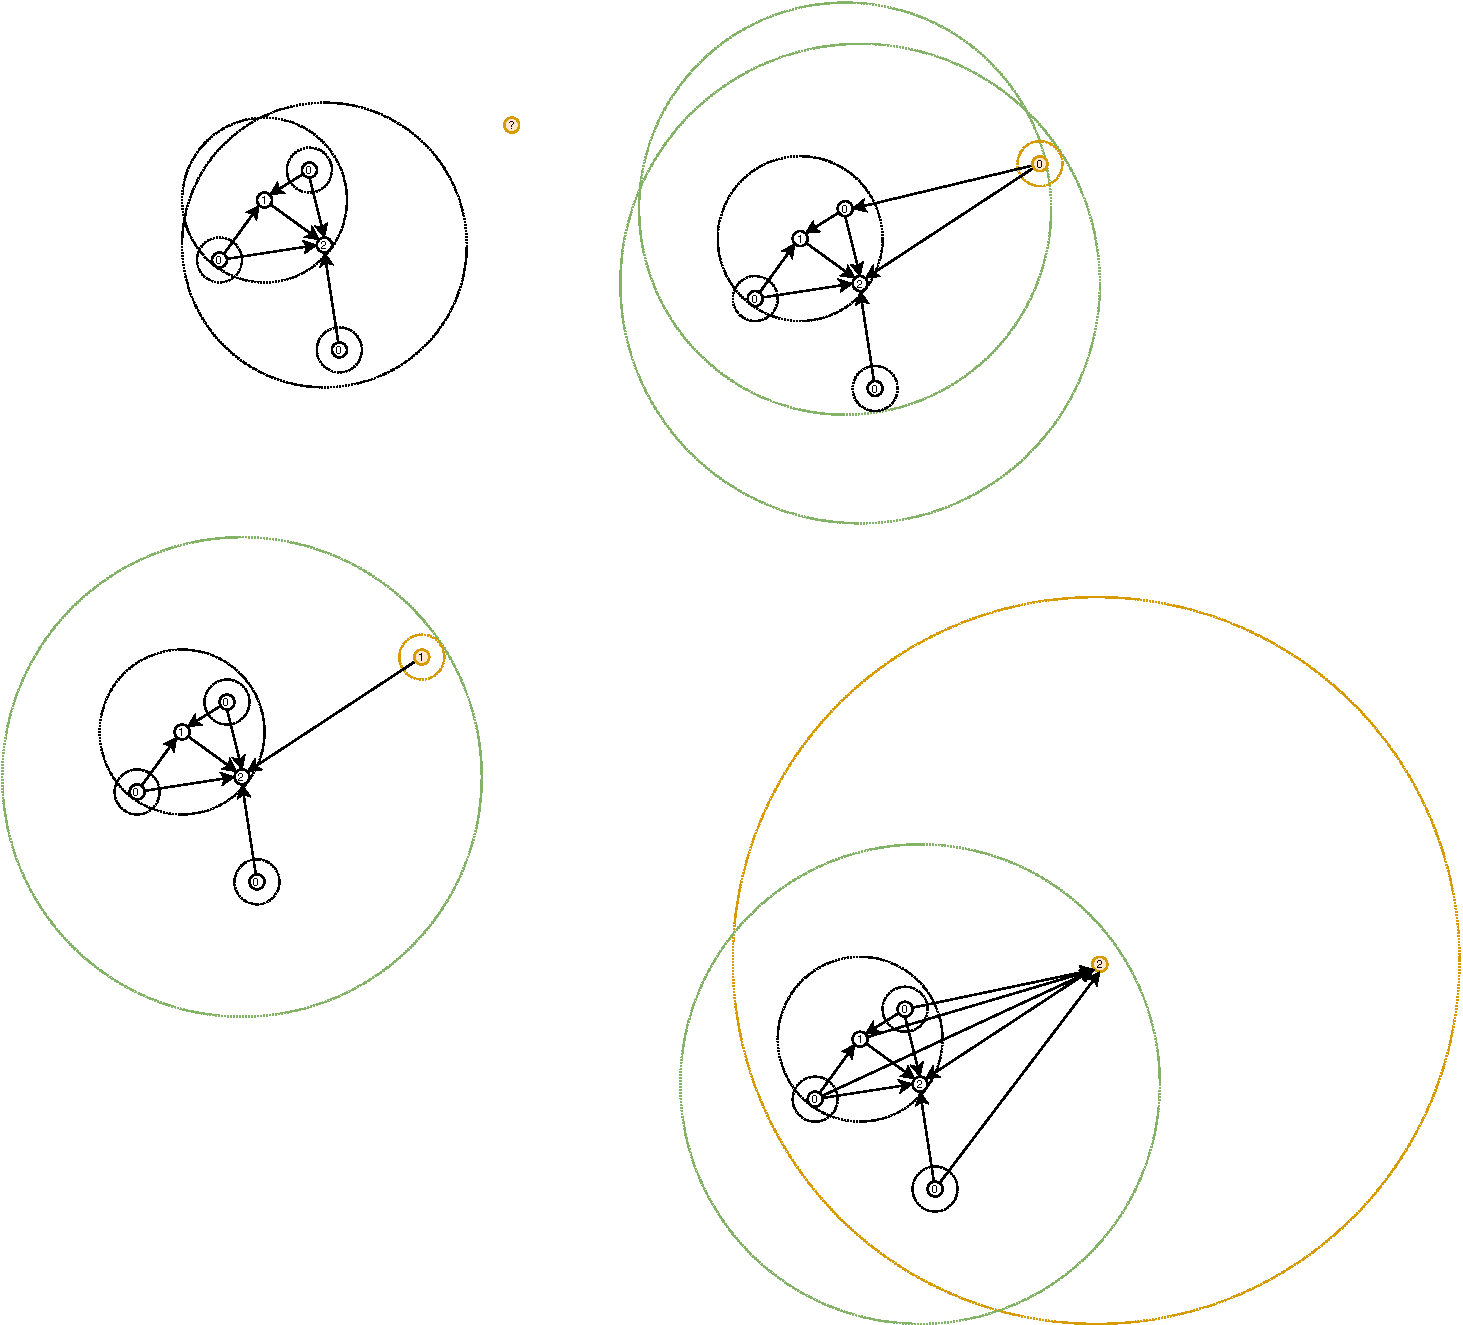
\includegraphics[width=300pt]{figures/LocarnoTreaties-Insertion-far}
\caption{Keeping the same level leads to smaller changes when a node enter the
  system. Shrinking regions are depicted in red, growing regions in green and
  same region in black.} \label{fig:LocarnoTreaties-Insertion-far}
\end{figure}

\subsection{Protocol}
The protocol is mostly the same as the simple control plane protocol
[\autoref{fig:registrationprotocol}]. The main difference is the level
assignment which follows the new algorithm described in \autoref{rebalancing}. 

\subsection{Threat Model}

The new lottery process can be targeted by attackers. If one malicious alone
decide to attack the system, it will not create too bad consequences, as it is
presented in \autoref{sec:ControlePlane-Threat-Model}. Another attack could be
that malicious nodes exit and reenter the system at each epoch until they
manage to get a good number from the lottery. Then when it manages to get a
good level, they collectively move to one side of the system leaving good nodes
all at level-0 in the middle of the system. This will create a slight overhead
for the good nodes as the region’s assignment increase for the level-0 nodes.
But this attack seems to cost a lot of resources and coordination for the
attacker to generate a small overhead on the size of the participants. Some
defence mechanisms can be set up to ensure that levels are geographically
distributed over the whole system, they are described in more details in
\autoref{chap:Possible Improvements}.

\subsubsection{Quantifying the Effect of Locarno Treaties}
The goal of the new protocol is to keep most regions and region assignment
following the evolution of the system. A concrete comparison is made. The
system starts with a fixed number of nodes and evolves with nodes moving,
leaving and entering the system. A quantity is chosen to evaluate the
difference between the system from one epoch to the next. The quantity is
defined as follows: the list of participants in the system is taken sorted by
name. Then for each node, their bunch and cluster will be compared. Each
difference will be counted, if a new node enters the system, their bunch and
cluster count as a difference. Same if a node leaves the system. The idea is
that with this new protocol, the total number of differences should be reduced.
The results of the experiment can be seen in [FIG.
\autoref{fig:LocarnoTreaties-differences}]. Maps of the system are given in
\autoref{app:LocarnoTreaties-data}.

\begin{figure}[!h] \centering
    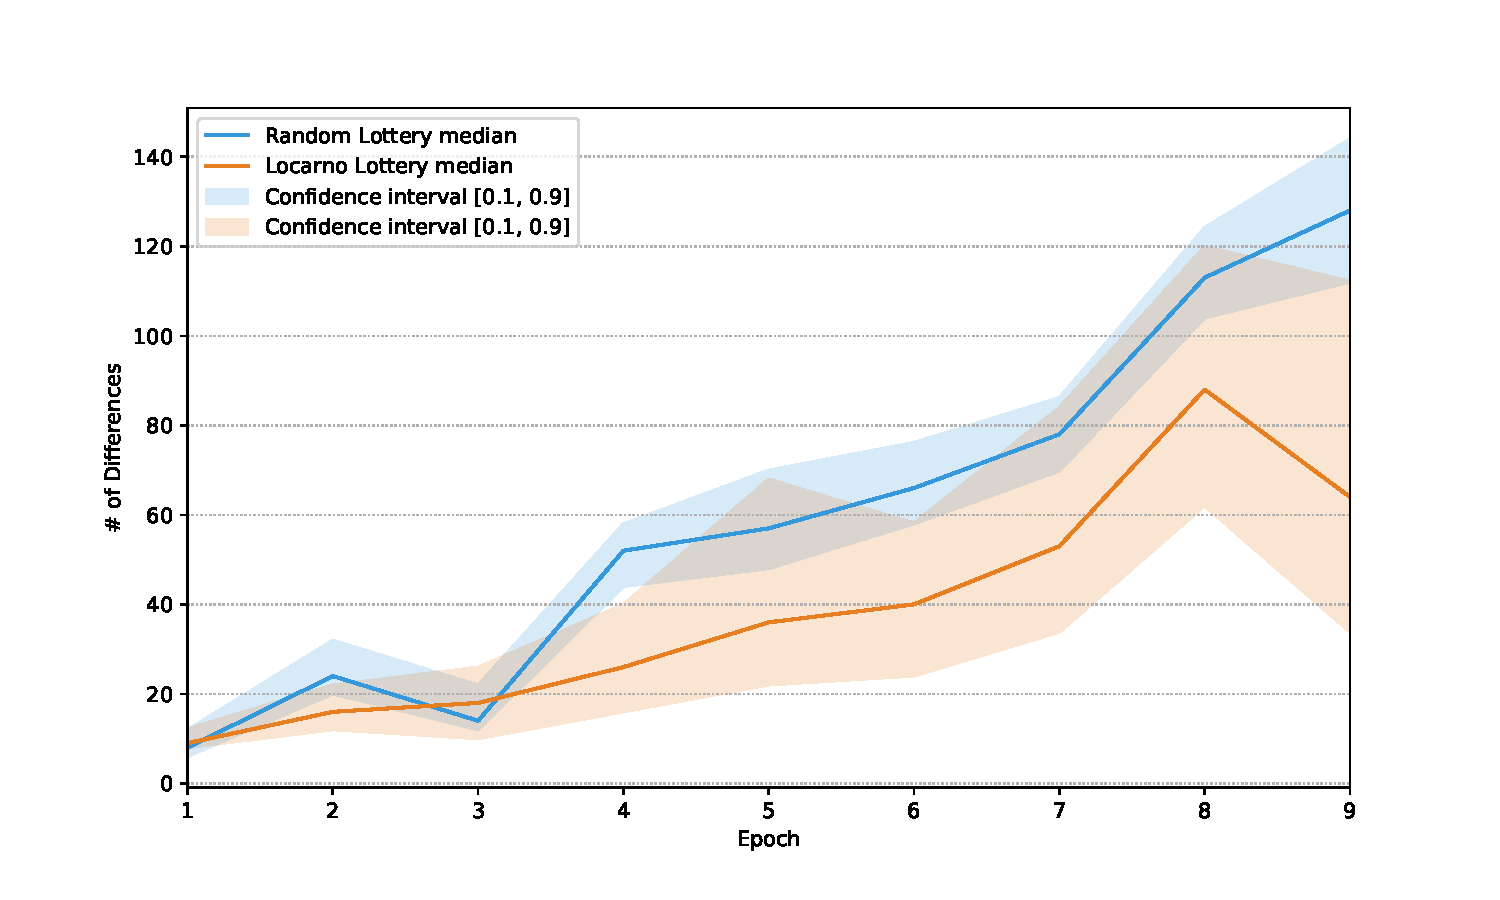
\includegraphics[width=300pt]{figures/LocarnoTreaties-differences}
    \caption{Graph of the number of differences between maps from one epoch to
    the next using the random level assignments or the one defined in Locarno
    Treaties. } \label{fig:LocarnoTreaties-differences} \end{figure}

\section{Strawman 2 : Fog of the War} \label{sec:Fog-of-the-war}

Each node of the system will have a different view of the world at a given time
depending on its place in the system and its interactions. Again the idea is
that one node should only be aware of the information it needs to perform its
actions. Correspondence can be made with the fog of war in some traditional
real-time strategy video game, where each player will have its view of the
system, based on where it is now (light), where it was in the past but cannot
see now (fog) and what it has not already seen (dark)
[\autoref{fig:fog-of-the-war}].  Each player view will evolve through space and
time accordingly. In the context of the game, the advantage of this view is
that it hides the adversarial strategy. In the context of our system, this view
will hide most of the information that is not relevant to one node but allow it
to perform its operation without the storage and communication overhead. 

The design of this Strawman will be the following. Each node declares a
position during the registration, and other nodes compute their bunch and
cluster according to this declared position. Each node will, therefore, be able
to compute their bunch and cluster based on these declared positions. To ensure
the correctness of the system a random committee of checkers is elected after
the registration process. These checkers will perform some tests (pinging other
nodes of one region) and publish the results. 

\begin{figure}[!h] 
\centering
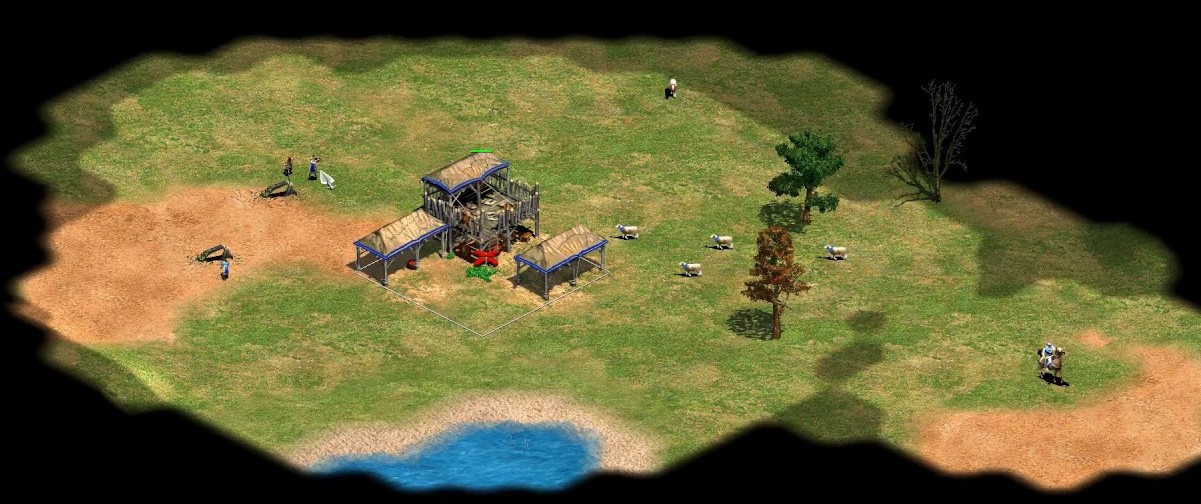
\includegraphics[width=400pt]{figures/fog_of_war}
\caption{Fog of war representation in a classic real-time strategy video game. }
\label{fig:fog-of-the-war}
\end{figure}

\subsection{Purpose : Reducing the Need of the Consensus on Distances}
The protocol presented in the Simple Control Plane protocol and the Locarno
Treaties still need a consensus on the distances between all nodes in the system.
This can be cumbersome as the number of nodes increases in the system this
quantity increases in $O(N^2)$, where $N$ is the number of nodes. Consensus
might become too costly for that reason.

The idea is to change that consensus with a declared position and a random
committee of checkers. The question is still: how to choose the committee? If
sampled randomly the chances are big that the selected nodes will be far away
from the node that they are supposed to check, and above a certain threshold,
the correlation between pings and distances are not satisfactory
\cite{Katz-bassett2006}. Therefore the committee of checkers can be selected to
be the $n$ closest nodes based on the declared distances. And $n$ can be
adapted to increase if one node does not pass the checks. 

If a node does not pass the checks, it either means that this node is faulty or
that the number of checkers is constituted of a majority of malicious nodes.
One can solve the second problem by increasing the number of checkers $n$, and
progressively a majority of honest nodes should have checked the node. It the
ping still does not correspond to what the node declared then one might assume
that the node itself is faulty. 

\subsection{Protocol}
The protocol is mostly the same as the simple control plane protocol
[\autoref{fig:registrationprotocol}]. The only difference is the consensus on
the pings which are now replaced by a declared distance, which is announced
before the level assignment and a round of checks and announce of the checks. 

\subsection{Threat Model}
Another question can be, what are we supposed to do with a node that is not
passing the tests? First, it is important to notice that it won't change the
view that all nodes will have of the system, as nodes use the declared distance
to compute their bunch and cluster. But one node could use that system to keep
its level and virtually go to a strategic place where it can unbalance the
system.  This is what one may want to avoid. 

There are three approaches to this problem, the first is to exclude the node
from the system, but it might lead to the redrawing of a certain number of
regions. Another strategy could be to define the position of the faulty node
with an approximation based on the ping. If we have the position of the other
nodes and we have to fix the location of the unknown faulty node one might do
that by computing the intersection between the circles based on the pings. This
triangulation strategy [\autoref{fig:triangulation_strategy}] can block one
faulty node to reach the desired position. 

\begin{figure}[!h] \centering
    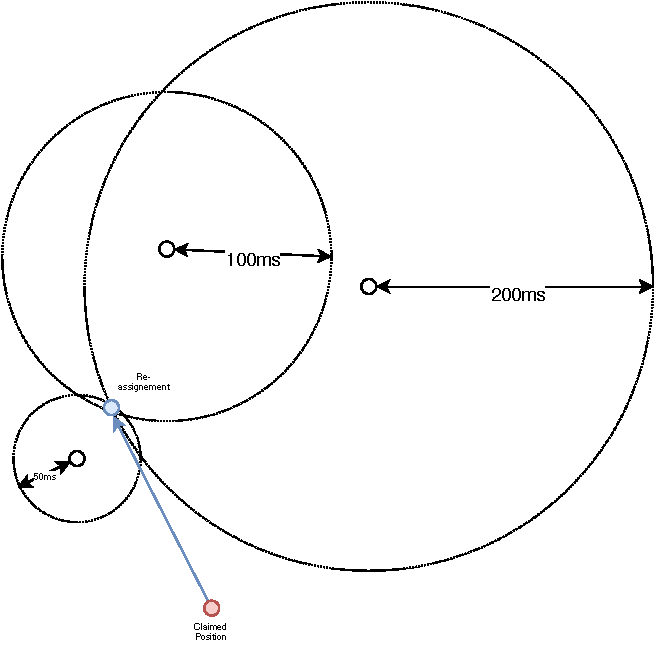
\includegraphics[width=300pt]{figures/triangulation_strategy}
    \caption{Triangulation can be used to reassign the position of a faulty
    node. }
\label{fig:triangulation_strategy}
\end{figure}

As nodes can announce a position and that is checked in priority by close
nodes, with this protocol if there is a sufficient number of malicious nodes,
they can declare that they all live in a close region and valid each other.
There is no simple solution to this problem, but that fact has no important consequences
on the system so it seems to be an acceptable weakness.

\section{Introducing the Space/Time Interaction distance}
One of the principal reasons to split the system based on the locality is
because of most regular transactions between people are local, therefore one
wants to ensure that in case of a global partition, most of the transactions
can still be processed flawlessly. The first idea for the locality was the
following. As there should be more interaction in local regions, most
interactions can be processed locally. This means that by using locality the
real goal is to maintain the interactions between the nodes. In that case,
the space metric is used to get an insight into the number of interactions
between nodes. And this is a reasonable approximation, but it might be worth it
to use directly theses interactions. 

\subsection{Interactions as a Distance on Space/Time Graphs}

If one wants to leverage the locality of interactions to build regions, it
might be worth it to investigate the following case. Imagine that some nodes
$A$ and $B$ interact often, but they are not part of the same local
region. By design, there is a bigger region in which they interact, and each of
these interactions should pass by this bigger region. One property that might
be useful is that these frequent interactions should have an impact on the
system leading to the creation or update of a region to include the interacting nodes. If the
metric that defines distance is changed from kilometres to "interactions". One
should be able to redraw the whole system based on that and to apply Crux to
create regions. Now how to define this metric? Let's try with the
following definition of distance :


$\forall A, B \in S$
\begin{equation} \label{definition-distance}
  d(A,B) = \frac{1}{ \mathrm{\#\ messages\ between\ A\ and\ B\ per\ unit\ of\ time} } 
\end{equation}
Where $S$ is the set of nodes in the system.

Interestingly this quantity as the property of a distance but not a metric
\cite{Greenhoe2016}. The properties of a metric and distances are listed below.
Indeed for the first, if we define that the number of messages that one node
sends to itself is infinite, the distance from one node to itself would be
zero. Second, the number of messages is positive meaning that the distance will
always be positive. Third, the interactions are counted as symmetric (if $A$ is
sending a message to $B$ we count that as an interaction between $A$ and $B$).
But for the fourth, the triangle inequality is not respected and that is a
problem indeed one should notice that if $A$ is close to $B$ and $B$ to $C$ but
$A$ and $C$ may never interact therefore are "far from each other".  

\paragraph{Properties} The properties of a metric are $1, 2, 4$ which implies
$3$. The properties of a distance is $1,2,3$ but not necessarily $4$
\cite{Greenhoe2016}. In the case of the interaction distance
\autoref{definition-distance}, $4$ is not respected.

$\forall A,B \in S$
\begin{enumerate}
\item $d(A,B) = 0 \Leftrightarrow A = B$
\item $d(A,B) \geq 0$
\item $d(A,B) = d(B,A)$
 \color{red} \item$d(A, C) \leq d(A,B) + d(B,C)$ \color{black}
\end{enumerate}

\paragraph{Example : CFF Distance}
A parallel can be made with the CFF distance. Indeed in some case, it is much
faster to take a train from $A$ to $B$ and then to take a train from $B$ to $C$
than taking a bus from $A$ to $C$ [\autoref{fig:CFF-map}][\autoref{fig:CFF-NewDistances}] . 

\begin{figure}[!h] 
\centering
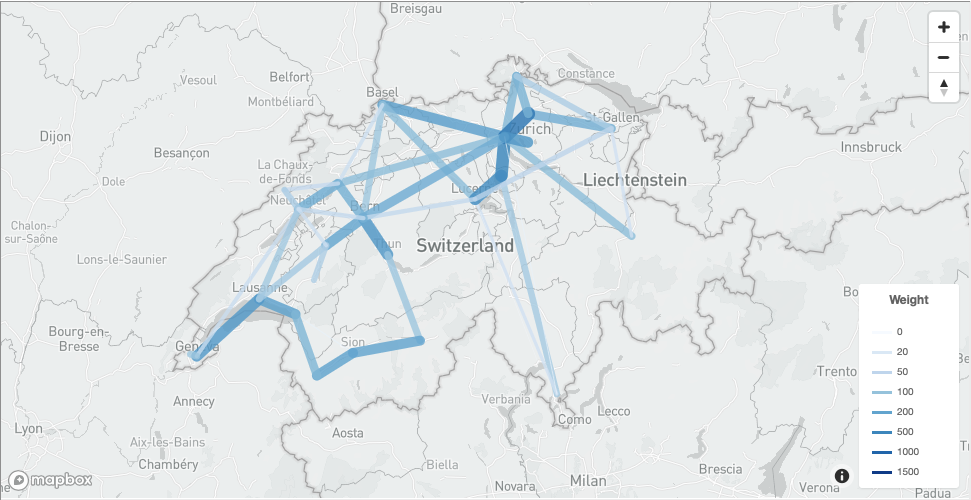
\includegraphics[width=450pt]{figures/CFF-map}
\caption{Map of the train network in Switzerland, line width is proportional to
  the number of connections per day.} \label{fig:CFF-map}
\end{figure}

\begin{figure}[!h] 
\centering
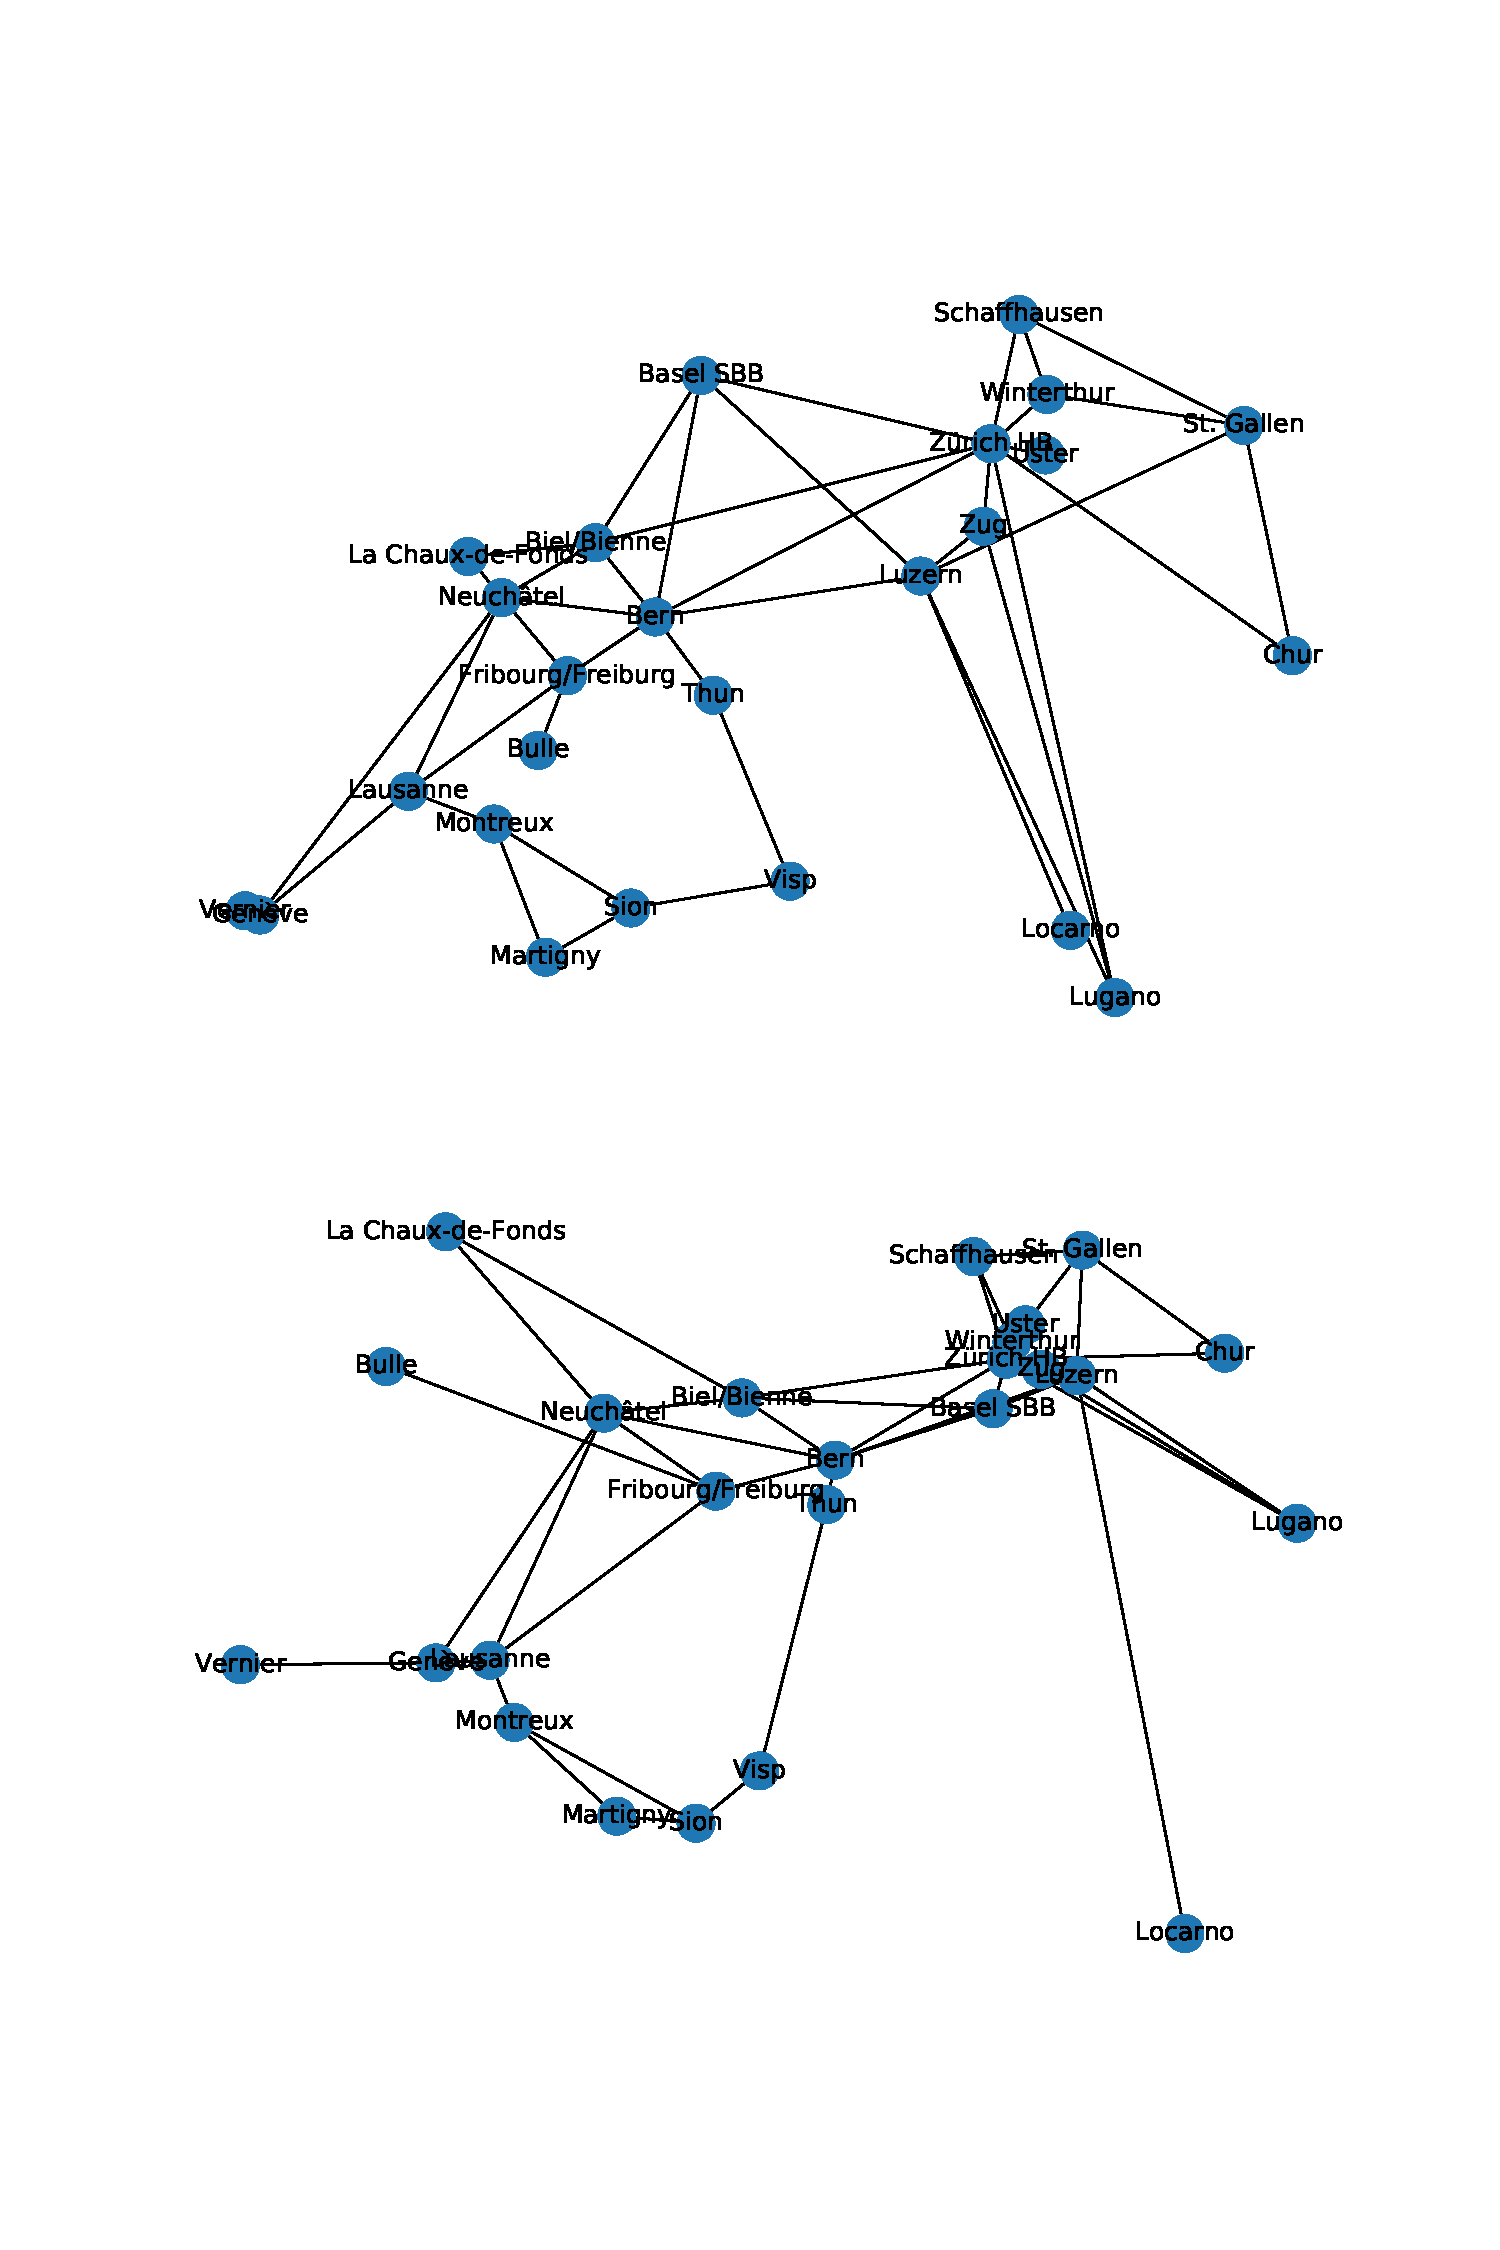
\includegraphics[width=350pt]{figures/CFF-NewDistances}
\caption{The train network is drawn again, using the regular distance first. In
  the second time the graph is displayed using the interaction distance as
  force in a force-directed graph. Ensuring that nodes that are close with
  regard to the interaction distance is close on the graph.}
  \label{fig:CFF-NewDistances}
\end{figure}

The fact that this new quantity is a distance and not a metric does not create
a problem in our case. Indeed all nodes are considering directly their distances
to all the other nodes in the system. When using the pings, nodes were required
to compute their pings to any other node in the system. Replacing that with the
interaction distance does not change anything. Triangle inequality could be
useful it one was trying to find a path from $A$ to $B$ and was considering
going by different other nodes to arrive at its goal. In our case this is not
the case, the hypothesis is that nodes have a one-to-one communication system.
Therefore it's only required to know the distance between any pair of points.

\subsection{Finding Meaning}
To understand better what this distance means, some examples are
considered. We want to understand what is meant to move with that new distance as
well as joining and leaving the system. 

\paragraph{Movements for Nodes With Interaction Distance}
It is easier to understand what it means to move in that space by looking to
the relative distance between nodes. Imagine that node $A$ get closer to node
$B$ but away from $C$ in that space. That means that the interactions between
$A$ and $B$ increases and on the contrary that the interaction between $A$ and
$C$ decreases.

\paragraph{Joining nodes with Interaction distance}
If a node joins the system and starts to interact with others, this can be
viewed as a node coming from infinity and getting closer to other
nodes.

\paragraph{Churning nodes with Interaction distance}
If a node churns and stops answering the other, this can be interpreted as a
movement in the interaction space. It is equivalent as if the churning nodes moved
to infinity.  

\paragraph{"Regions" With Interaction Distance} \label{par:section-example}
The concept of the "region" is harder to conceive with that new notion of
distance. It might be useful to use the parallel with the CFF
\autoref{fig:CFF-NewDistances}, let's imagine a node at EPFL and try to
conceptualize to what might correspond the equivalent of "local", "regional"
and "global regions". The "local" region might be depicted with what places can
be reached within 15 min of public transportation. This will cover the metro
line to Lausanne and some bus stops. At the regional level, it might be what
places are reachable within 1 hour of public transportation. The global region still
covers all the nodes.

\subsection{Justification to Replace the Locality}
Changing the distance from the regular one to interactions might have some
implication on the property that we want to keep in the system. 

\paragraph{Partition Resistance}
Even more than preserving working regions
composed of geographically close nodes it might be more interesting to preserve
the set of nodes that have a lot of interactions. As this might be the nodes
that are doing the most operations of the system. This justifies the use of
this new distance.

\paragraph{Region Validation for Transaction}
One problem that Nyle wanted to solve was region validation, to allow fast
processing of transactions. This is still possible in that case. However, the
region does not correspond to the same anymore. But they would correspond to
the example depicted in \autoref{par:section-example}. This might be acceptable
for a client. 

\subsection{Protocol}
The protocol is the same as the one described in Locarno Treaties at
\autoref{Locarno}. The only difference is that the distance is changed by the
new distance [\autoref{definition-distance}]. The computation of the number of
messages is done in the following way: Each node keeps the track of the count
of messages it receives from other nodes between epochs, and post the results
at the beginning of the next epoch instead of the pings. Each node is able then
to compute the new distance, and the algorithm for regions can be used
directly. In the first epoch, as nodes did not have the time to interact a lot
with each other, pings are used instead of the interaction distance.


%%%%%%%%%%%%%%%%%%%%%%%%%%%%%%%%%%%%%%%%%%%%%%
\chapter{Possible Improvements} \label{chap:Possible Improvements} %%%%%%%%%%%
%%%%%%%%%%%%%%%%%%%%%%%%%%%%%%%%%%%%%%%%%%%%%%

This chapter lists the improvements that could be applied more or less directly
to one part of the project, but that was not implemented due to time reasons. 

In the simple control plane protocol, the live clock that is supposed to be
synchronised for every node could be replaced by Timestamps Logical Clocks (TLC)
\cite{Ford2019}. This could allow the system to be more flexible.
However, this was not implemented as it was hard to see how to go from one
epoch to another using TLC. Recall that in the existing protocol, at the
beginning of the live period one node of the old committee sends the necessary
information to the new committee to begin. Synchronising this with TLC could be hard.

One other improvement that can be added is to allow clients to ask for the
generation of regions with special meaning. For example, it could make sense to
create a region that is corresponding to precise geographical areas. This could
allow the client to precisely know where its transactions are validated. For
example, it could mean more to him to know that his transaction is validated in
Swiss and Western Europe but not yet globally than knowing that its transaction
is validated in some local area but not globally. 

One of the assumptions that were taken is that the distribution of the levels
would be geographically distributed at random. And that will be the case as the
nodes are supposed to be as well geographically distributed at random.
However, it was stated that this aspect could be targeted by malicious nodes.
To avoid that attack, some mechanisms could be developed to ensure
that the levels are geographically distributed at random. One approach could be
to compute the density of levels per region and to detect if it is more or less
the same. If it diverges too much, a fall back to random attribution of levels
could be applied. 

\section{Roadmap}
Of course, this work is just a small part of what is left to do to have the first
version of Nyle. Here is a list of what is to implement to have the first version
of Nyle and description of the current progress.

\begin{itemize} 
\item Based on the location through time and space of nodes, build regions.
(Done in this work)
\item In each of the region of the regions build a Blockchain. (Could use an
  existing one.)
\item Use the transaction validation to give info on the validated region. (To
do) 
\item Dealing with moving actors. (Done in this work)
\item Manage the transfer of data from one epoch to the next (To do)
\item Dealing with double-spending issues. (To do)
(if a node spends the same coin in different regions). 
\end{itemize}

%%%%%%%%%%%%%%%%%%%%%%%%%%%%%%%%%%%%%%%%%%%%%%
\chapter{Conclusion} \label{chap:Conclusion} %%%%%%%%%%%%%%%%%%%%%%%
%%%%%%%%%%%%%%%%%%%%%%%%%%%%%%%%%%%%%%%%%%%%%%

%, In conclusion, you repeat the main result and finalize the discussion of
%your project. Mention the core results and why as well as how your system
%advances the status quo.

This works proposed a control plane for locality-preserving blockchains. First,
a simple version of the control plane was designed. This protocol splits the
time into epochs, containing a registration period and a live period. Nodes can
register for the next epoch by providing a valid \textit{endorsement} to the
participants of the current epoch during the registration period. The current
participants then proceed to generate consensus on the list of future
participants. At the beginning of the live period, all the pings between the
participants are computed and participants draw levels from a public source of
randomness, and the regions are created deterministically from the pings and
the levels. This first version is already reaching the goal that was expected
from the control plane, which is to deal with nodes entering, leaving and
moving in the system.  The threat analysis was done and it seems to be secure
given that no more than $f_i$ malicious nodes are in the system at any epoch
$i$, with $f_i$ given by $3f_i+1=N_i$ and where $N_i$ is the number of
participants at the epoch $i$.  However, it was demonstrated that this protocol
was consuming a lot of resources in memory and communication. 

A series of improvements were proposed. The first one, called \textit{Locarno
Treaties} proposed to change the system of a lottery to allow nodes to keep
their level, while ensuring that their final distribution was not unbalanced.
It was then shown that with this improvement, the differences from one epoch to
the next were reduced drastically. A second one, called \textit{Fog of the War}
was proposed to reduce the needs of communication. It is worked by changing the
map of all pings between participants in the system with a declared position,
which is then checked by a committee of checkers. The security analysis of this
improvement was done as well. But the implementation was not made due to time
reasons. 

A third improvement called \textit{Space/Time Interaction Distance} was
proposed as well. The idea of this improvement was to change the notion of
locality, from the regular interpretation of \textit{distance} to a new one.
With this new interpretation, nodes that are interacting a lot are viewed as
close. And in the opposite, nodes that do not communicate are separated with an
infinite distance. With the new interpretation, a node that churns is seen from
the others as a node which is moving towards infinity.  

%% TODO add amelioration 

%% Implementation + Mention the core results and why as well as how your system
%advances the status quo.
The implementation of the simple version of the control plane, the first and
the third Strawman was made in Go. It was done using the Cothority Framework
and based on an existing code base from Cristina Basescu. The evaluation was
made on Deterlab. This work enhances Nyle by proposing a control plane, which
is necessary as the system of nodes that will run Nyle is not supposed to be
stable. It should be possible for nodes to leave, join and move into the
system, which is made possible by the proposed control plane. Other
applications that are based on CRUX \cite{Basescu2014} might consider using
this work to ensure that nodes can move, churn or enter in the system.

It was a pleasure for me to do this work. Working with locality-preserving
blockchains allowed me to dive into the blockchain world and to discover a lot
of new technologies. Working with the Cothority Framework was an interesting
experience and it sharpened my programming skills by understanding more of the
concurrency. I found that the logic of decentralized and distributed systems
are complex but I find really interesting to develop protocols for these
systems. I want to thank my supervisor for the precious help during the
project.


\cleardoublepage \phantomsection \addcontentsline{toc}{chapter}{Bibliography}
\printbibliography


%%%%%%%%%%%%%%%%%%%%%%%%%%%%%%%%%%%%%%%%%%%%%%
\appendix %%%%%%%%%%%%%%%%%%%%%%%%%%%%%%%%%%%%%%%%%
%%%%%%%%%%%%%%%%%%%%%%%%%%%%%%%%%%%%%%%%%%%%%%

\chapter{Problems with levels}

\section{Problem with unbalanced levels } \label{app:unbalanced-levels}
The problem with unbalanced levels is mainly that a property stated in CRUX
\cite{Basescu2014} is not necessary respected anymore. The property is the
following : Let's call $ARAs_{max}$ the maximum number of regions in which a
node participates. This number is given by : 

\begin{equation} \label{eq:ARAmax}
ARAs_{max} = \log_2(R_{max}/R_{min}) (B \log_B(N)+1)
\end{equation}

Where $B$ is a constant, $N$ is the number of nodes in the system, $R_{min}$ is
the diameter of the smallest region and $R_{max}$ is a diameter that is large
enough to cover the entire network. This ensures that the overhead that is
created by the replication stays reasonable: by design, it is growing
logarithmically with the number of nodes $N$ and with $R_{max}$. We will
describe two situations where this property is not maintained, as an argument
for keeping the distribution of levels balanced.

\subsection{Problem With level-0 Nodes} \label{app:levels-zero}
Assume that there is a system of $N$ nodes that are all at level 0. If all
the nodes stay at level 0, by construction, they will have every other node in
their bunch [\autoref{fig:ClusterBunch-Bunch}]. (Because it’s adding every
other node if their level it not smaller.) After adding $N$ nodes with this
process, the $N$The node will participate in $N-1$ region which grows a lot
faster than \autoref{eq:ARAmax}. This could create an unmanageable overhead.
Therefore one needs to have higher-level nodes in the middle of levels 0 nodes.
This justifies the attack on levels that could be done by malicious nodes as
described in \autoref{sec:ControlePlane-Threat-Model}. And the solution
proposed in \autoref{chap:Possible Improvements}.

\subsection{Problem With Too Many Different Levels} Similarly consider the case
where we have $N$ nodes and each is at a different level from $0$ to $N-1$. By
design, the node at level $0$ will have every other node in its bunch. So it
will participate in $N$ regions, which grows a lot faster with $N$ than
\autoref{eq:ARAmax}. This could lead to an unmanageable overhead as well. Of
course, this example is a bit extreme, but it gives guidelines on what could
happen if the distribution of levels is not controlled.

\chapter{Locarno Treaties : Data} \label{app:LocarnoTreaties-data}

\begin{figure}[!h] 
\centering
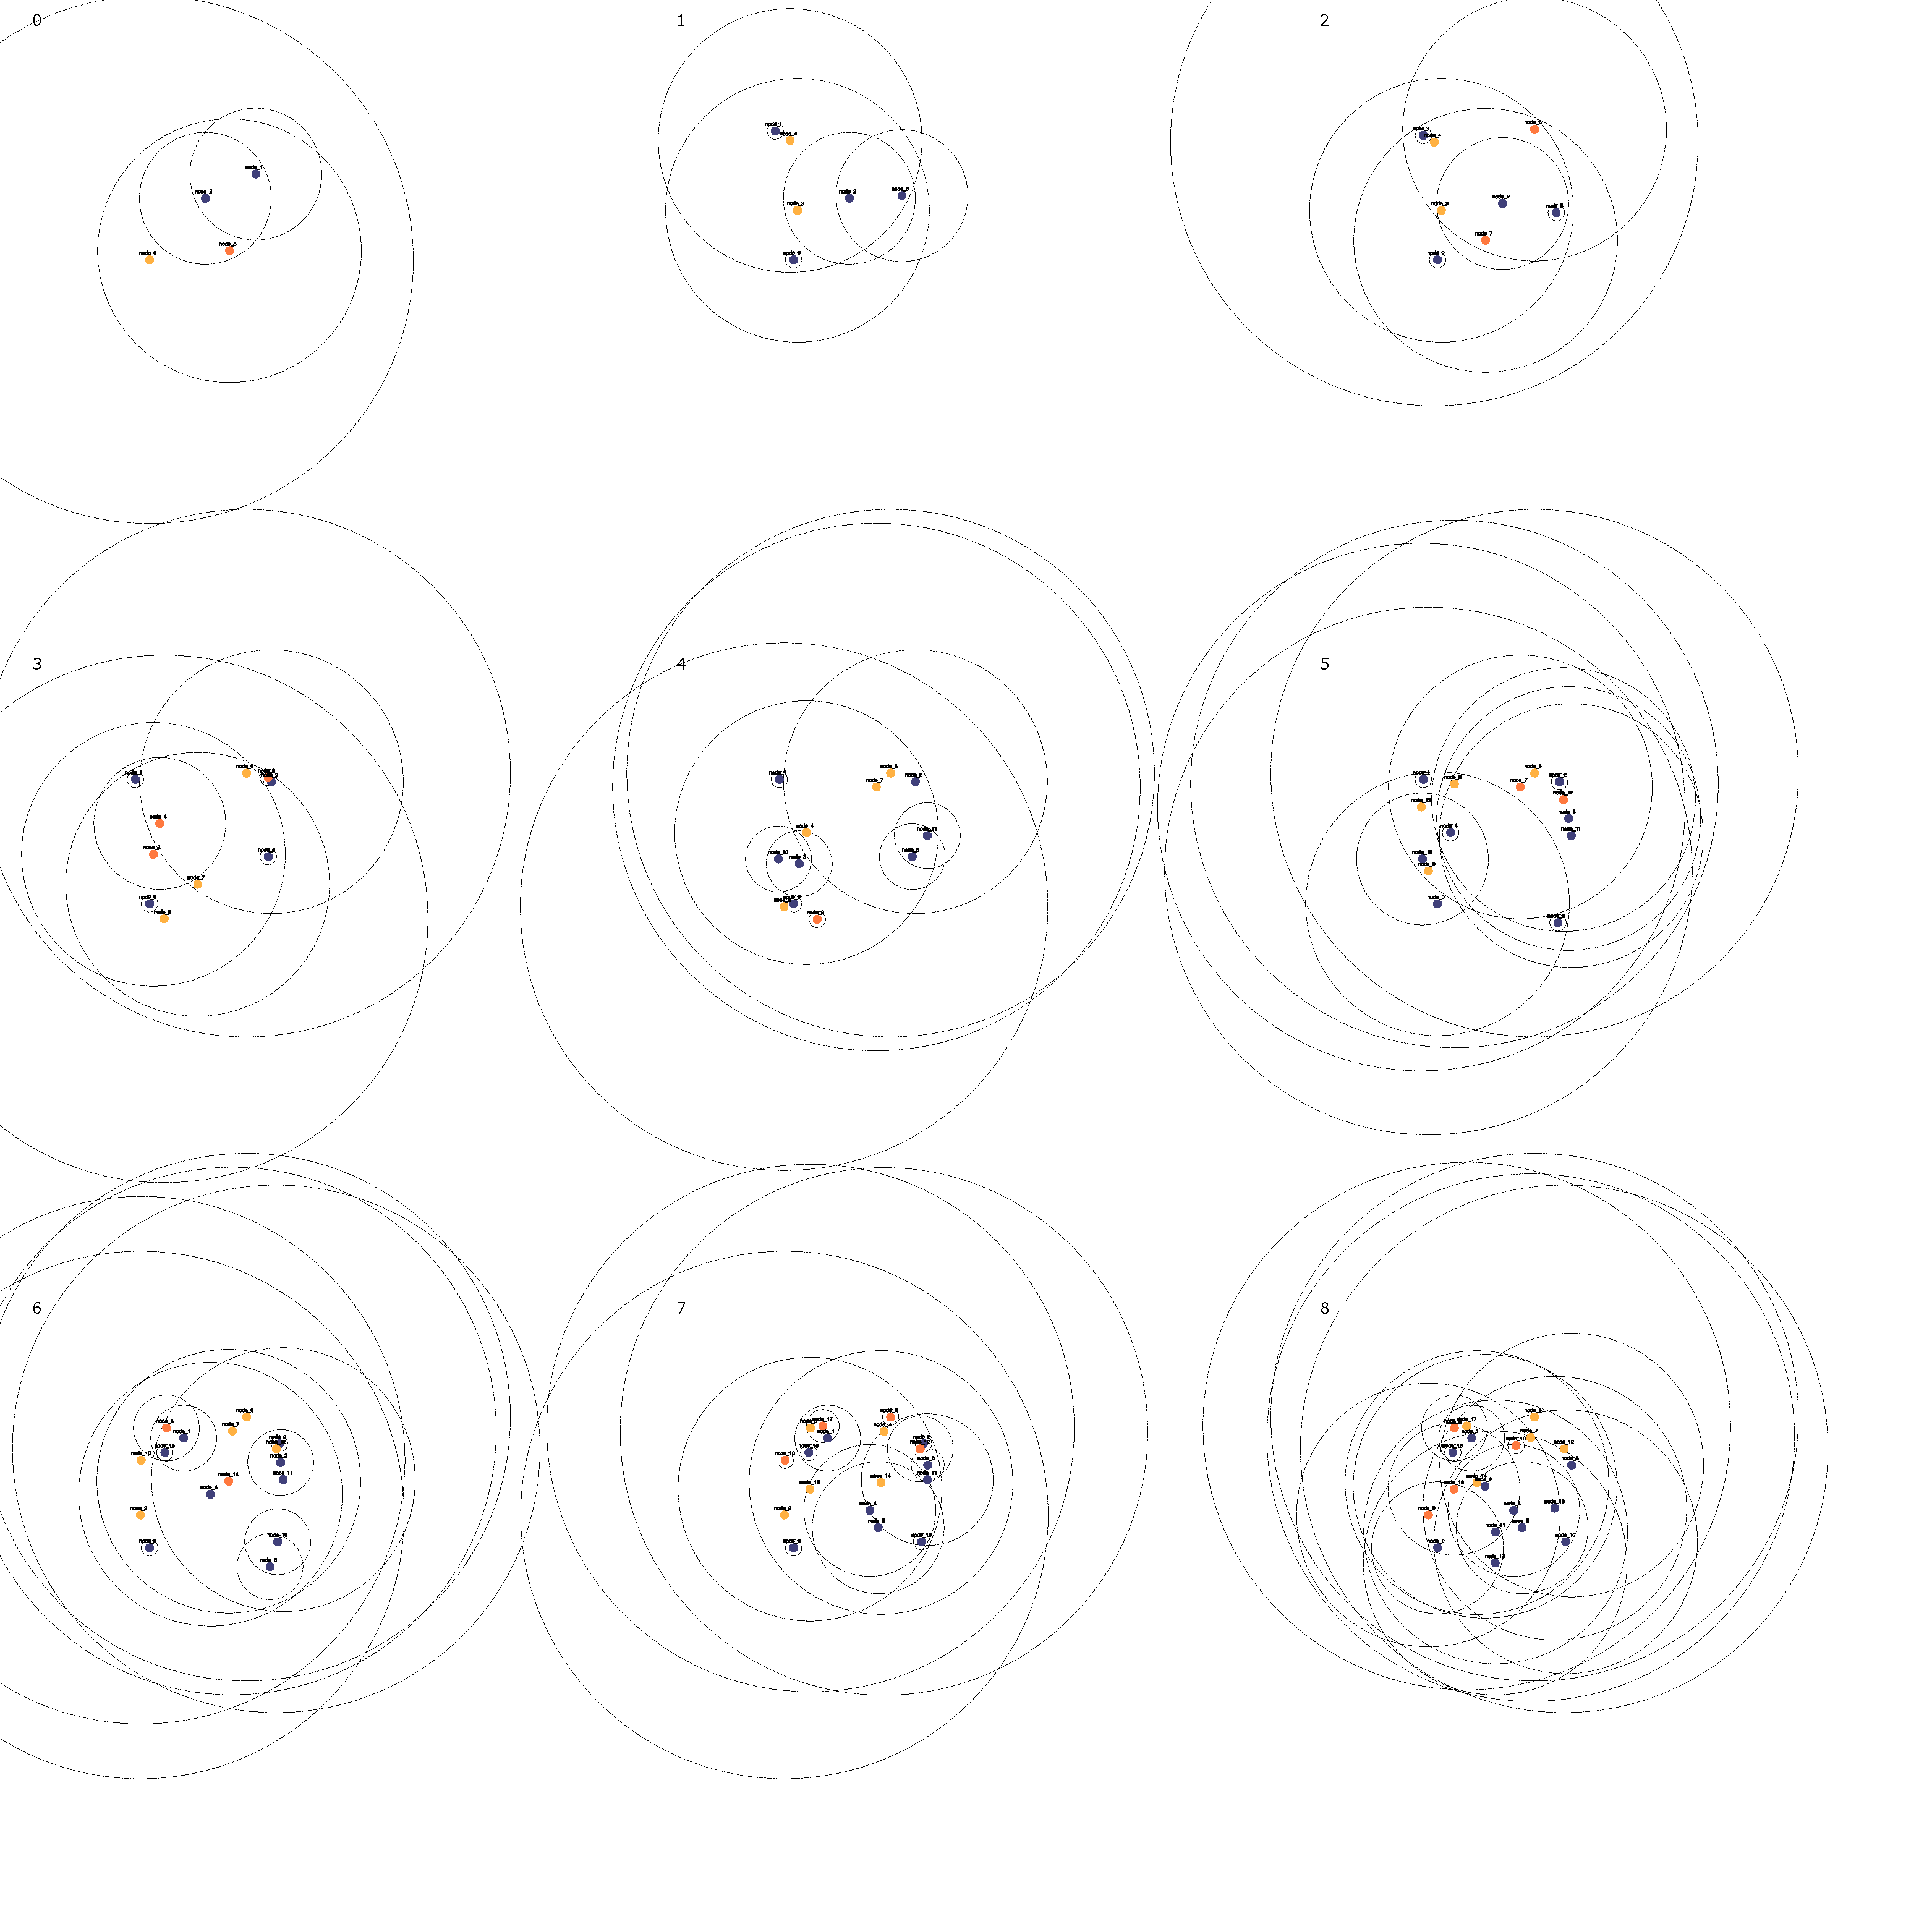
\includegraphics[width=350pt]{figures/LocarnoTreaties-RandomFinal}
\caption{Graphs of the system using random lottery at each epoch, the levels are depicted in different colors.}
\label{fig:LocarnoTreaties-RandomFinal}
\end{figure}

\begin{figure}[!h] 
\centering
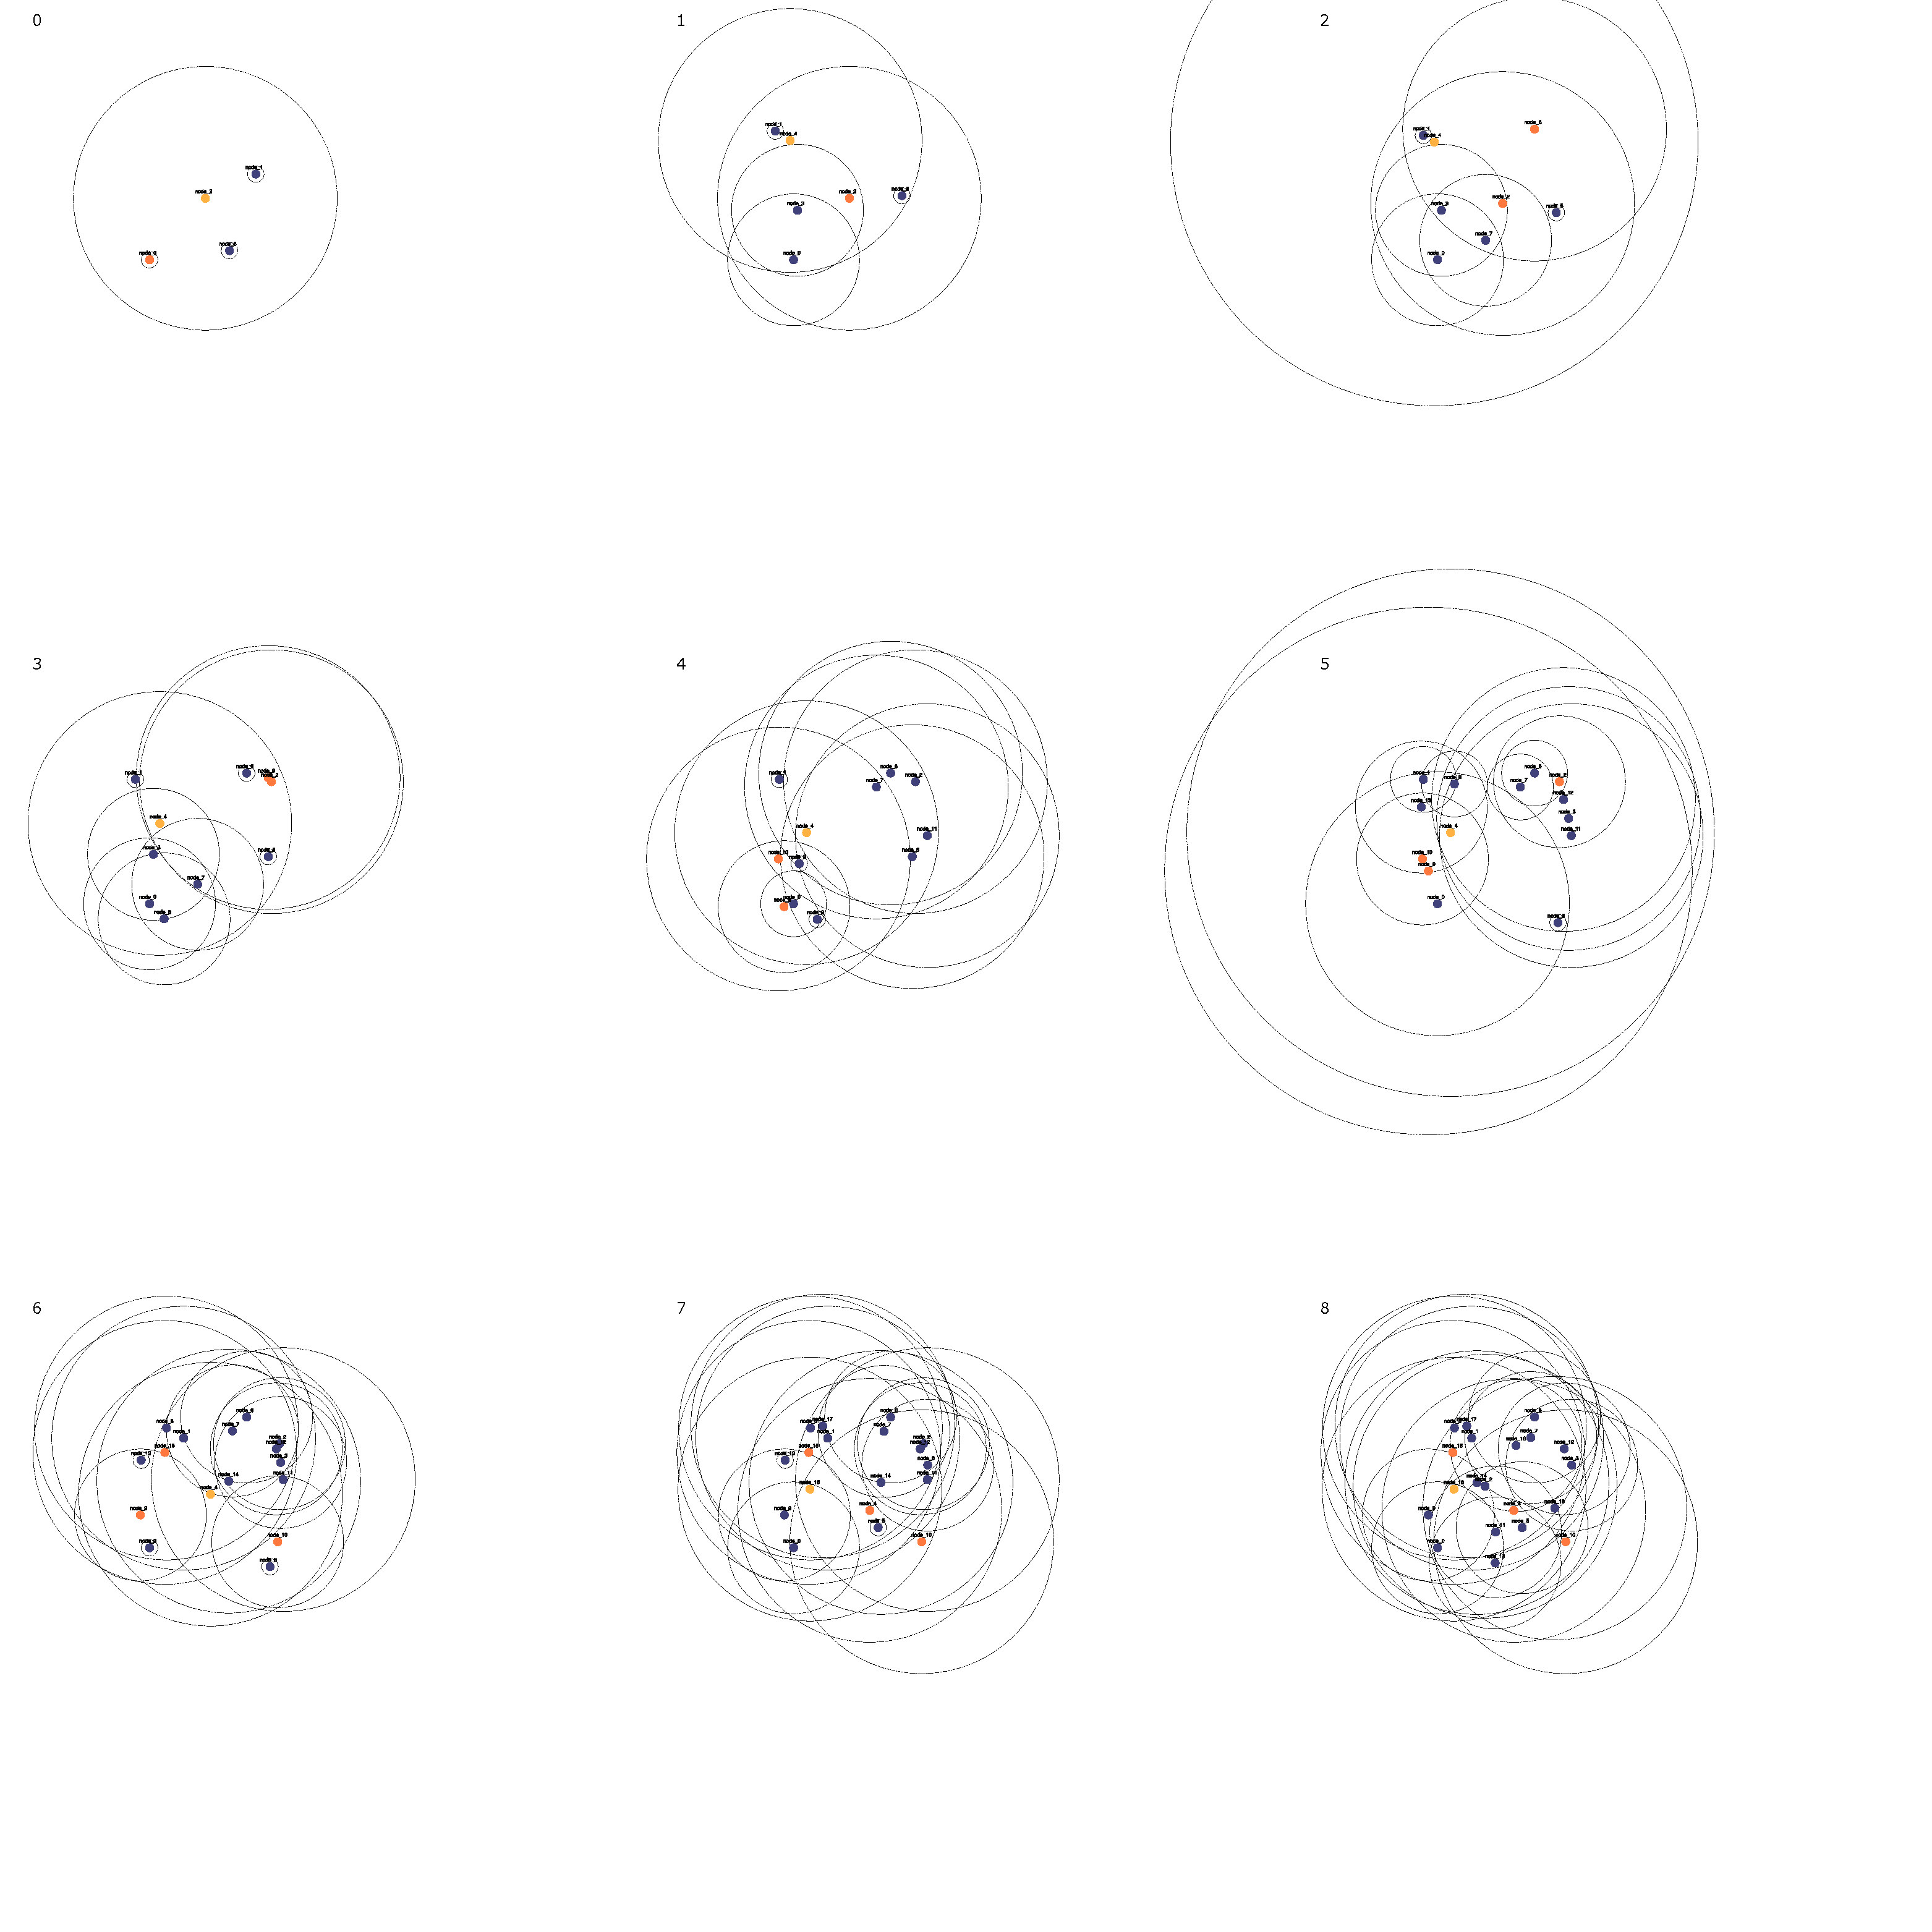
\includegraphics[width=500pt]{figures/LocarnoTreaties-LocarnoFinal}
\caption{Graphs of the system using \textit{Locarno Treaties} lottery at each
    epoch, the levels are depicted in different colors.}
    \label{fig:LocarnoTreaties-LocarnoFinal}
\end{figure}


\chapter{Dataset on Master Thesis}
Here are some important random facts about this master's thesis. The
aggregation of data was stopped the day of the printing.  \begin{table}[h]
\centering
\begin{tabular}{@{}lrrrr@{}}
\toprule
\textbf{Language}     &\textbf{Files} & \textbf{Blank} & \textbf{Comment} & \textbf{Code} \\ \midrule
Go        & 25  & 1'222 & 857   & 3'935 \\ \hdashline
SVG       & 9   & 0   & 0    & 1'587 \\ \hdashline
TeX       & 7   & 263  & 128   & 1'372 \\ \hdashline
Python      & 4   & 79  & 2    & 315 \\ \hdashline
Markdown     & 4   & 60  & 0    & 132 \\ \hdashline
Jupyter Notebook & 2   & 0   & 844   & 130 \\ \midrule
Total      & 56  & 1'645 & 1'832  & 7'525 \\
\midrule
\bottomrule
\end{tabular}
\caption{Line of code for the different languages used in that project}
\label{tab:my-table}
\end{table}

\begin{table}[h]
\centering
\begin{tabular}{@{}lr@{}}
\toprule
\textbf{Number of}       & \textbf{Total} \\ \midrule
 Commits & 148  \\ \hdashline
 Coffees & 249  \\ \hdashline
Days  & 82  \\ \hdashline
Graphs & 26  \\
\midrule
\bottomrule
\end{tabular}
\caption{Some random stats}.
\label{tab:my-table}
\end{table}


\end{document}
